\section{Experiments}\label{sec:experiments}

We evaluate \repay{} by simulation, first on synthetic traces and then on traces built from public measurements (Sections~\ref{sec:exp-real} and~\ref{sec:exp-real2}).
The questions are whether the theoretical guarantees are visible at realistic scales (Sections~\ref{sec:exp-bound} and~\ref{sec:exp-opt}), how the rule compares with common schedulers when devices are truthful (Section~\ref{sec:exp-compare}) and when they are not (Section~\ref{sec:exp-strategic}), how the comparison depends on the traffic mix and the population (Section~\ref{sec:exp-mix}), how it compares with further schedulers and fair-division rules from the literature (Section~\ref{sec:exp-baselines}), and what the business constraints and the solver cost (Sections~\ref{sec:exp-tiers} and~\ref{sec:exp-runtime}).
All code, seeds and result files are in the repository that accompanies the paper.\footnote{\url{https://github.com/vinhqdang/computer_network_optimization}}

\subsection{Setup}\label{sec:exp-setup}

\paragraph{Scenarios.}
A slot is one second and rates are in Mbit/s.
In the \emph{hotspot} scenario devices arrive as a Poisson process with rate $0.25$ per slot, with an additional batch of Poisson(12) arrivals every $180$ slots (a train or a flight), and stay for a geometric time with mean $240$ slots; about $75$ devices are present on average.
Tiers are drawn with probabilities $(0.6,0.25,0.15)$ for free, premium and PAYG, and classes with probabilities $(0.65,0.25,0.10)$ for elastic, video and gaming.
Elastic devices have a link rate uniform on $[5,30]$ and alternate between active and idle periods (a two-state Markov chain with mean durations $50$ and $20$ slots); while active their demand cap is the link rate, so the link is saturated whenever elastic devices are active.
Capacity is $150$~Mbit/s modulated by a three-state Markov chain with multipliers $(1,0.6,0.2)$ and mean holding time $33$ slots, times lognormal noise; the mean is about $91$~Mbit/s, so the fair share per device moves between roughly $2$ and $0.4$~Mbit/s, above and below the minimum video rate.
In the \emph{home} scenario ten premium devices share $25$~Mbit/s with the same modulation; calls and game sessions start and end at random.
The utilities are those of Section~\ref{sec:model} with $\rmin_{\mathrm{v}}=0.5$, $\rmax_{\mathrm{v}}=3$, $r_{\mathrm{g}}=0.2$; weights are $w_F=1$, $w_P=2$, $w_Y=1.5$; committed rates are $c_P=2$ and $c_Y=1.5$ with $\theta_P=0.8$, $\theta_Y=0.6$, $\phi=0.15$; and $V=20$ unless stated otherwise. The tier queues use the normalisation of Section~\ref{sec:algorithm}, with $\bar C$ the mean capacity of the trace.

\paragraph{Baselines.}
\textsc{PF} is class-blind weighted proportional fairness, recomputed every slot, with RT flows capped at $\rmax_k$.
\textsc{WFQ} is the same with the weights of declared RT flows multiplied by four.
\textsc{Priority} serves declared RT flows first, with admission control: flows are admitted at $\rmin_k$ in order of tier (premium, PAYG, free), gaming before video, and arrival, while capacity lasts, admitted video flows then share what is left up to $\rmax_{\mathrm{v}}$, and elastic devices receive the remainder by weighted proportional fairness.
\textsc{Plain DPP} is drift-plus-penalty with the same utilities and tier queues as \repay{} but without deficit queues; it represents utility-maximising schedulers that know the classes.
\textsc{Credit} is a class-blind credit scheduler in the spirit of Karma~\citep{vuppalapati2023karma}: every device has a weighted fair share, devices that use less than their share earn credit, and spare capacity goes to the borrowers with the most credit. It is our adaptation to this setting, not the original system.
We also run the three variants of Section~\ref{sec:variants}, and Section~\ref{sec:exp-baselines} adds six further baselines.

\paragraph{Metrics.}
\emph{RT success} is the fraction of slots of genuine RT flows in which the flow receives at least $\rmin_k$.
\emph{Elastic rate} is the mean rate of genuine elastic devices while active.
\emph{Utility} is the sum over devices of their true per-slot utility, averaged over time.
\emph{Class envy} is computed in the same way for every rule, from realised rates: for each elastic device we track the largest window sum of (mean rate of the RT flows of its tier, capped at its own demand, minus its own rate), and report the maximum over devices.
Unless stated otherwise we report means over seeds with 95\% confidence intervals based on Student's $t$ quantiles; with three to ten seeds these intervals are indicative, and since all rules run on the same traces we also give paired differences where a comparison matters.
The number of independent traces is $10$ for the comparison and the additional baselines; $5$ for the bound, the trade-off curves, the call continuity, the variability sweep, the sweep over the real-time share and the binding-constraint table; $3$ for the default business constraints, the optimality gap and the population sweep; $4$ for the collapse curves and the short stays; $6$ for the unilateral deviations and the switching and oracle attacks; and $2$ for the reverse deviation, the oracle ablation and the deviations under capped priority, under the additional baselines and at a low real-time share. Runs last $6000$ slots for the comparisons and $3000$ for the strategic experiments, from an empty system and without warm-up.
Capacity noise is lognormal with $\sigma=0.15$ and sojourns last at least five slots. All traces are synthetic except in Sections~\ref{sec:exp-real} and~\ref{sec:exp-real2}.

\subsection{The envy bound}\label{sec:exp-bound}

Figure~\ref{fig:bound}(a) shows the largest deficit observed in any slot, for any device and class, relative to its bound $B_{g,k}$, over five seeds of $6000$ slots.
Besides the hotspot scenario we use an adversarial capacity trace that alternates between $150$ and $15$~Mbit/s every $60$ slots.
The ratio never exceeds $0.46$, in line with Theorem~\ref{thm:bound} and Remark~\ref{rem:sharp}.
Figure~\ref{fig:bound}(b) shows what the bound buys.
Without deficit queues the same drift-plus-penalty rule produces class envy between $535$ and $1012$~Mbit; with them the envy stays between $2.7$ and $58$~Mbit and below the theoretical line.
On the hotspot the price is in RT success: at $V=20$ \repay{} serves $92.4\%$ of video slots against $99.9\%$ for plain DPP, and at $V=100$ $99.0\%$ against $100\%$, while at $V=20$ elastic devices receive $16\%$ more ($1.66$ against $1.43$~Mbit/s).

\paragraph{How large is the bound?}
Table~\ref{tab:bsize} puts the video bound next to what elastic devices actually receive, for the $180$ devices of Section~\ref{sec:exp-strategic} (stays of at least $60$ slots, median about $200$).
At $V=20$ the bound is between a sixth and a little over a quarter of the volume a device receives during a median stay, and the largest realised envy is four to ten times smaller than the bound.
For a stay of $60$ slots the bound is close to the whole volume received, and for the shortest stays it says nothing; Section~\ref{sec:exp-strategic} therefore tests short stays separately.
An operator can read the choice of $V$ off this table: $V$ is the envy bound, in units of $w_g\eta_k$, that it is willing to tolerate, and it should be small compared with the volume of the stays it wants to protect.

\begin{table}[t]
\centering
\caption{The video bound $B_{g,\mathrm{v}}=Vw_g\eta_{\mathrm{v}}+\rmax_{\mathrm{v}}$ at $V=20$ against realised quantities under \repay{} ($180$ elastic devices on six traces, truthful declarations). The gaming bounds are $100$, $200$ and $150$~Mbit.}
\label{tab:bsize}
\resizebox{\linewidth}{!}{\begin{tabular}{lrrrrr}
\toprule
Tier & $B_{g,\mathrm{v}}$ (Mbit) & Median volume of a stay (Mbit) & Median $B/$volume & Median realised envy (Mbit) & Largest realised envy (Mbit) \\
\midrule
Free & 43 & 196 & 0.22 & 7.9 & 11.7 \\
Premium & 83 & 491 & 0.17 & 5.3 & 8.7 \\
PAYG & 63 & 225 & 0.28 & 7.9 & 11.5 \\
\bottomrule
\end{tabular}}
\end{table}

\begin{figure}[t]
\centering
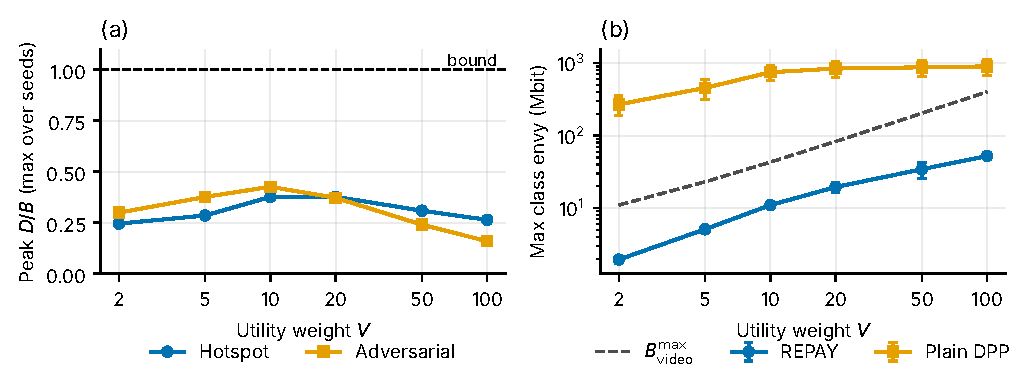
\includegraphics[width=\linewidth]{figures/fig_bound.pdf}
\caption{(a) Largest deficit relative to the bound of Theorem~\ref{thm:bound} (maximum over seeds). (b) Maximum class envy of \repay{} and of the same rule without deficit queues; the dashed line is the largest video bound $\max_gB_{g,\mathrm{v}}$.}
\label{fig:bound}
\end{figure}

\subsection{Optimality gap}\label{sec:exp-opt}

To test Theorem~\ref{thm:opt} we fix a population (two tiers, three video flows, one gaming flow and five elastic devices with different demand caps), draw the capacity independently in each slot from $200$ equally likely values (sampled once from a mixture of lognormals with medians $30$, $12$ and $4$~Mbit/s), and compute the benchmark $U^*$ of \eqref{eq:bench} with a conic solver (with $\theta_P=0.5$ and $\phi=0.15$; three seeds for the simulation).
Both tier constraints turn out to be slack on this instance, so the gap is governed by the envy constraints, which enter the benchmark through the affine majorant; utility here is the operator's weighted objective.
Its value is $18.13$. Without the envy constraints the optimum is $18.22$, and with envy-freeness imposed in every slot instead of on average it drops to $17.78$: on this instance the whole value of time-shifting is $0.35$ and the cost of class-envy-freeness, once time-shifting is allowed, is $0.09$.
Figure~\ref{fig:optgap} shows the time-average fluid utility of \repay{} over $20\,000$ slots.
The gap to $U^*$ is $0.44$ at $V=5$, $0.091$ at $V=20$ and $0.030$ at $V=100$; the product of gap and $V$ lies between $1.82$ and $3.03$ for $V\ge5$, consistent with a gap of order $1/V$ (the constant $B_0$ of Theorem~\ref{thm:opt} is far larger than these values, so the bound itself is not tight), and already at $V=10$ \repay{} is above the slot-wise envy-free optimum, so it does exploit time-shifting.
Plain DPP reaches slightly more than $U^*$ because it ignores the envy constraints; class-blind PF obtains $17.52$.
The largest deficit in these runs is $0.21$ of its bound.

\begin{figure}[t]
\centering
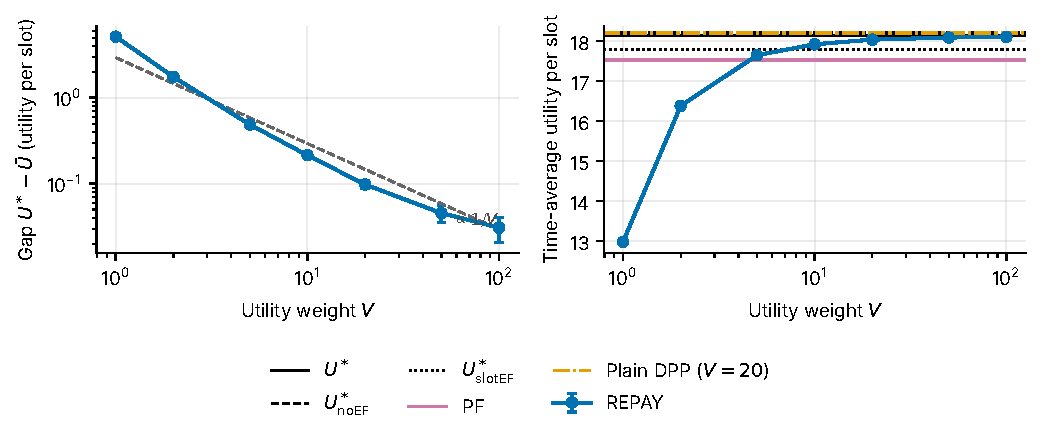
\includegraphics[width=\linewidth]{figures/fig_optgap.pdf}
\caption{Optimality gap on a fixed population with i.i.d.\ capacity. Left: gap to the benchmark $U^*$ against $V$. Right: average utility against the three benchmark values.}
\label{fig:optgap}
\end{figure}

\subsection{Comparison with truthful devices}\label{sec:exp-compare}

Table~\ref{tab:compare} and Figure~\ref{fig:compare} compare all rules on the hotspot scenario when every device declares its true class ($10$ seeds, $6000$ slots).
The rules fall into three groups.
\textsc{WFQ} and \textsc{Priority} serve nearly all RT slots, but they do so by taking capacity from elastic devices for good: the elastic rate falls from about $1.75$ to $1.26$--$1.27$~Mbit/s and class envy reaches $2000$ to $2200$~Mbit; plain DPP serves $99.9\%$ of RT slots with an elastic rate of $1.52$~Mbit/s and class envy of $1070$~Mbit.
\textsc{PF} and \textsc{Credit} are fair to elastic devices and leave RT flows unprotected ($82$--$83\%$ of RT slots, $76$--$80\%$ for video).
\repay{} serves $95.0\%$ of RT slots while giving elastic devices almost what \textsc{PF} gives them ($1.74$ against $1.78$~Mbit/s) and keeping class envy at $15$~Mbit.
It closes $72\%$ of the gap in RT success between \textsc{PF} and \textsc{Priority} at a $2.3\%$ lower elastic rate and with a higher utility than \textsc{PF}.
The intervals in the table overlap because the traces differ more than the rules do; the paired differences between \repay{} and \textsc{PF} over the ten traces are $+13.1\pm1.3$ points of RT success, $+3.9\pm0.3$ in utility and $-0.040\pm0.004$~Mbit/s in elastic rate, each with the same sign on every trace.
Plain DPP, which differs from \repay{} only by the deficit queues, serves $4.9\pm1.3$ points more RT slots and has a utility higher by $2.2\pm0.3$, with an elastic rate lower by $0.23$~Mbit/s ($13\%$): this is the price of bounded envy when everyone is truthful.
The utility figures add real-time and elastic utilities on the scales of Section~\ref{sec:model}, so their ranking depends on that exchange rate; RT success and elastic rate do not.
The gain is in the free tier, where $92\%$ of RT slots are served against $70\%$ under \textsc{PF}; the paid tiers are served in more than $99\%$ of slots by every rule except \textsc{Credit} ($95\%$ for premium and $84\%$ for PAYG). These per-tier figures are computed from the result files and are not in the table.
When all devices are truthful, \textsc{Priority}, plain DPP and \textsc{WFQ} have the highest utility ($74.8$, $74.7$ and $74.0$ against $72.6$ for \repay{}); their defects are envy and, as Section~\ref{sec:exp-strategic} shows, incentives.
\textsc{Repay-WC} coincides with \repay{} in every run, so its recycling condition (spare capacity while every elastic device is at its cap) has no effect in any run and the variant is not exercised by our experiments. \textsc{Repay-E} differs by at most $0.01$ in utility and $0.1$ point in video success: the entrant offer matters when a tier has no RT flow, which is rare with $75$ devices.
Dropping the debt price (No-debt) raises RT success by $2.6\pm0.5$ points and class envy from $15$ to $25$~Mbit, at an elastic rate lower by $0.025$~Mbit/s.

In the home scenario capacity is ample most of the time and all rules serve $97\%$ of RT slots or more (Table~\ref{tab:compare-home}); the differences are again in class envy, $10$~Mbit for \repay{} against $165$ for plain DPP and $460$ for \textsc{WFQ} and \textsc{Priority}, which coincide on this scenario because RT flows never have to be rationed.

\begin{table}[t]
\centering
\caption{Hotspot scenario, truthful devices (mean over 10 seeds, $\pm$ half-width of the 95\% confidence interval). Premium and PAYG ratios are served volume over committed demand and the free-floor ratio is served volume over the floor; the targets are $0.8$, $0.6$ and $1$. Utility is the unweighted sum of true utilities.}
\label{tab:compare}
\resizebox{\linewidth}{!}{% Source: results/compare.json, scenario hotspot
\begin{tabular}{lrrrrrrrrrr}
\toprule
Mechanism & Utility & RT success (\%) & Video success (\%) & Elastic rate (Mbit/s) & Jain index & Premium ratio & PAYG ratio & Free-floor ratio & Max class envy (Mbit) & 95th-pct.\ device envy (Mbit) \\
\midrule
REPAY & 72.6 $\pm$ 2.4 & 95.0 $\pm$ 1.3 & 93.1 $\pm$ 1.8 & 1.74 & 0.791 & 1.32 & 1.29 & 2.90 & 14.6 $\pm$ 1.5 & 11.4 \\
REPAY-WC & 72.6 $\pm$ 2.4 & 95.0 $\pm$ 1.3 & 93.1 $\pm$ 1.8 & 1.74 & 0.791 & 1.32 & 1.29 & 2.90 & 14.6 $\pm$ 1.5 & 11.4 \\
REPAY-E & 72.6 $\pm$ 2.4 & 95.0 $\pm$ 1.3 & 93.0 $\pm$ 1.8 & 1.74 & 0.791 & 1.32 & 1.30 & 2.90 & 14.6 $\pm$ 1.5 & 11.4 \\
No-debt & 73.6 $\pm$ 2.4 & 97.6 $\pm$ 1.0 & 96.7 $\pm$ 1.4 & 1.72 & 0.787 & 1.22 & 1.24 & 3.15 & 25.1 $\pm$ 0.5 & 23.4 \\
Plain DPP & 74.7 $\pm$ 2.3 & 99.9 $\pm$ 0.1 & 99.9 $\pm$ 0.2 & 1.52 & 0.707 & 1.35 & 1.30 & 2.85 & 1072.1 $\pm$ 163.0 & 370.6 \\
PF & 68.7 $\pm$ 2.6 & 81.9 $\pm$ 2.2 & 79.8 $\pm$ 2.3 & 1.78 & 0.783 & 1.44 & 1.36 & 2.62 & 0.0 $\pm$ 0.0 & 0.0 \\
WFQ & 73.9 $\pm$ 2.2 & 98.7 $\pm$ 0.6 & 98.2 $\pm$ 0.8 & 1.27 & 0.630 & 1.22 & 1.25 & 3.14 & 1980.6 $\pm$ 290.2 & 708.9 \\
Priority & 74.8 $\pm$ 2.3 & 100.0 $\pm$ 0.0 & 100.0 $\pm$ 0.0 & 1.26 & 0.625 & 1.15 & 1.22 & 3.31 & 2211.7 $\pm$ 328.7 & 763.8 \\
Credit & 64.4 $\pm$ 2.5 & 82.6 $\pm$ 2.5 & 75.7 $\pm$ 3.1 & 1.87 & 0.800 & 1.21 & 1.24 & 3.17 & 127.4 $\pm$ 28.4 & 35.6 \\
\bottomrule
\end{tabular}
}
\end{table}

\begin{table}[t]
\centering
\caption{Home scenario, truthful devices (mean over 10 seeds).}
\label{tab:compare-home}
\resizebox{0.85\linewidth}{!}{% Source: results/compare.json, scenario home
\begin{tabular}{lrrrrrrrr}
\toprule
Mechanism & Utility & RT success (\%) & Video success (\%) & Elastic rate (Mbit/s) & Jain index & Premium ratio & Max class envy (Mbit) & 95th-pct.\ device envy (Mbit) \\
\midrule
REPAY & 7.9 $\pm$ 0.3 & 100.0 $\pm$ 0.0 & 100.0 $\pm$ 0.0 & 3.19 & 0.998 & 1.47 & 10.3 $\pm$ 2.2 & 10.3 \\
REPAY-WC & 7.9 $\pm$ 0.3 & 100.0 $\pm$ 0.0 & 100.0 $\pm$ 0.0 & 3.19 & 0.998 & 1.47 & 10.3 $\pm$ 2.2 & 10.3 \\
REPAY-E & 7.8 $\pm$ 0.3 & 100.0 $\pm$ 0.0 & 100.0 $\pm$ 0.0 & 3.19 & 0.998 & 1.47 & 10.2 $\pm$ 2.2 & 10.1 \\
No-debt & 7.9 $\pm$ 0.3 & 100.0 $\pm$ 0.0 & 100.0 $\pm$ 0.0 & 3.18 & 0.998 & 1.47 & 24.2 $\pm$ 2.5 & 24.2 \\
Plain DPP & 7.9 $\pm$ 0.3 & 100.0 $\pm$ 0.0 & 100.0 $\pm$ 0.0 & 3.13 & 0.997 & 1.47 & 164.5 $\pm$ 37.3 & 163.1 \\
PF & 7.8 $\pm$ 0.3 & 99.3 $\pm$ 0.5 & 99.1 $\pm$ 0.6 & 3.20 & 0.998 & 1.47 & 0.0 $\pm$ 0.0 & 0.0 \\
WFQ & 7.8 $\pm$ 0.3 & 100.0 $\pm$ 0.0 & 100.0 $\pm$ 0.0 & 3.05 & 0.997 & 1.47 & 459.4 $\pm$ 143.6 & 447.2 \\
Priority & 7.8 $\pm$ 0.3 & 100.0 $\pm$ 0.0 & 100.0 $\pm$ 0.0 & 3.05 & 0.997 & 1.47 & 459.4 $\pm$ 143.6 & 447.2 \\
Credit & 7.6 $\pm$ 0.3 & 97.0 $\pm$ 2.4 & 96.1 $\pm$ 2.6 & 3.18 & 0.998 & 1.47 & 120.1 $\pm$ 37.9 & 115.7 \\
\bottomrule
\end{tabular}
}
\end{table}

\begin{figure}[t]
\centering
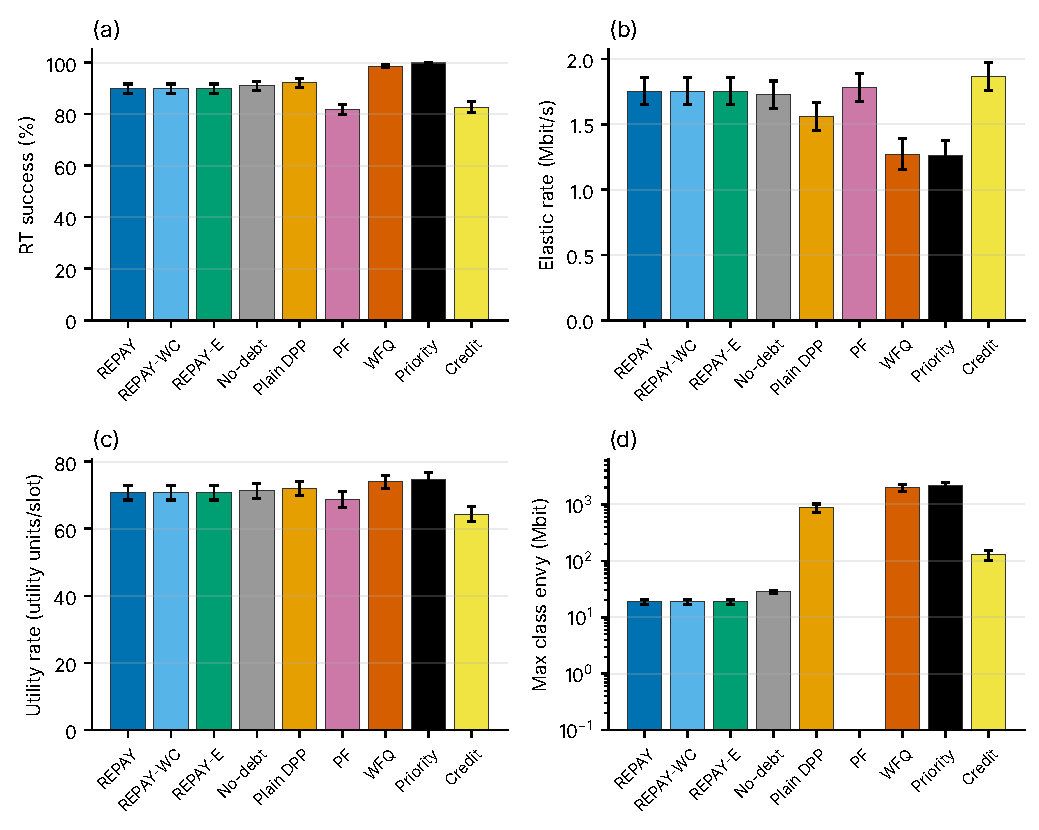
\includegraphics[width=0.9\linewidth]{figures/fig_compare.pdf}
\caption{Hotspot scenario, truthful devices: (a) RT success, (b) elastic rate, (c) utility, (d) maximum class envy (logarithmic scale; \textsc{PF} has none).}
\label{fig:compare}
\end{figure}

\paragraph{Trade-off curves and a capped priority.}
Each rule has a parameter that moves it between protecting RT flows and serving elastic devices, and a single setting can flatter or penalise it.
Figure~\ref{fig:frontier} therefore sweeps $V$ for \repay{} and plain DPP and the RT weight multiplier for \textsc{WFQ}, on five traces.
We also add a baseline that a practitioner would try first, \emph{capped priority}: strict priority in which declared RT flows may use at most a fraction $q$ of the capacity of the slot, so that the reward for declaring RT is limited by construction.
\repay{} lies to the right of plain DPP and \textsc{WFQ} at every level of RT success, that is, it protects the same share of RT slots while leaving more to elastic devices.
Capped priority, however, does better than \repay{} on this pair of metrics around $q=0.3$: there it serves $93.2\%$ of RT slots with an elastic rate of $1.80$~Mbit/s, against $92.3\%$ and $1.67$ for \repay{} at $V=10$ and $94.4\%$ and $1.66$ at $V=20$, because it holds admitted calls close to their minimum rate; its utility is lower ($70.1$ against $71.9$ for \repay{} at $V=20$). At $q=0.5$ it is below the curve of \repay{} ($99.5\%$ at $1.46$~Mbit/s, against $99.3\%$ at $1.63$ for \repay{} at $V=100$).
Table~\ref{tab:cap} shows what it gives up.
Its class envy is $390$~Mbit at $q=0.3$, about $28$ times that of \repay{} at $V=20$, and grows quickly with $q$; and its resistance to misreporting depends on the cap being tight for the traffic mix at hand: with $q=0.2$ or $0.3$ a misreporting device loses on average and $2\%$ or $25\%$ of the devices gain, fewer than under \repay{} on the same $60$ devices ($58\%$, median change $+1.5\%$); with $q=0.5$ the median device gains $69\%$.
When the share of real-time devices falls from $35\%$ to $10\%$, the same cap $q=0.3$ no longer binds and the median misreporting device gains $113\%$, against $-0.9\%$ under \repay{} (Section~\ref{sec:exp-mix}); the right cap thus depends on the share of real-time traffic, which the operator does not know and which changes during the day, whereas $V$ sets the envy bound whatever the mix.
We read this as follows. If an operator only needs calls to survive short shortages, knows its traffic mix and can tune a cap, capped priority is a simple and effective answer, and the case for \repay{} rests on what it guarantees to each elastic device, not on average performance.

\begin{figure}[t]
\centering
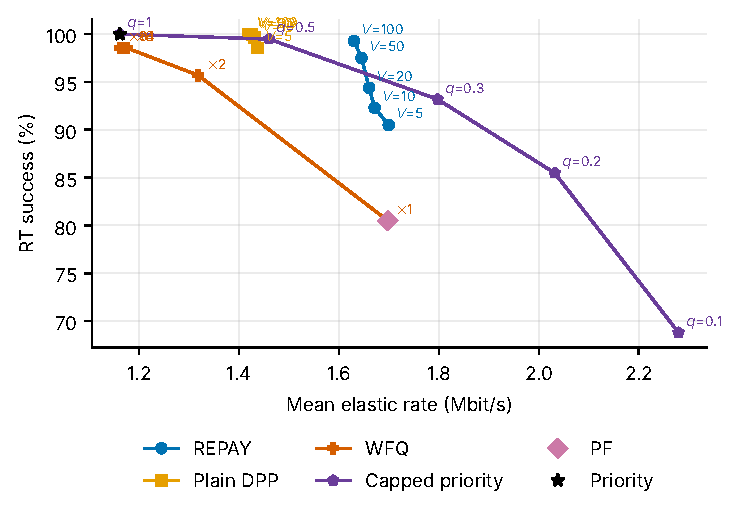
\includegraphics[width=0.7\linewidth]{figures/fig_frontier.pdf}
\caption{RT success against elastic rate when the parameter of each rule is varied (hotspot, truthful devices, mean over five traces).}
\label{fig:frontier}
\end{figure}

\begin{table}[t]
\centering
\caption{Capped priority: RT flows may use at most a fraction $q$ of capacity. Left columns: truthful devices, five traces. Right columns: one elastic device declares video ($60$ devices on two traces, as in Section~\ref{sec:exp-strategic}).}
\label{tab:cap}
\resizebox{\linewidth}{!}{% Source: results/frontier.json; truthful columns mean $\pm$ 95% CI half-width over seeds (hotspot, T=6000); deviation columns from the unilateral static deviation (T=3000, seeds 0 and 1)
\begin{tabular}{rrrrrrr}
\toprule
$q$ & RT success (\%) & Elastic rate (Mbit/s) & Max class envy (Mbit) & Median rel.\ gain of misreport (\%) & Pooled volume gain (\%) & Devices gaining (\%) \\
\midrule
0.1 & 68.8 $\pm$ 1.0 & 2.28 $\pm$ 0.14 & 1.57 $\pm$ 2.65 & -- & -- & -- \\
0.2 & 85.5 $\pm$ 1.0 & 2.03 $\pm$ 0.12 & 67.97 $\pm$ 49.92 & -55.33 & -60.40 & 1.7 \\
0.3 & 93.2 $\pm$ 1.2 & 1.80 $\pm$ 0.11 & 390.66 $\pm$ 169.75 & -20.27 & -33.03 & 25.0 \\
0.5 & 99.5 $\pm$ 0.4 & 1.46 $\pm$ 0.08 & 1296.82 $\pm$ 216.89 & 68.74 & 27.02 & 66.7 \\
1 & 100.0 $\pm$ 0.0 & 1.16 $\pm$ 0.06 & 2065.24 $\pm$ 593.74 & -- & -- & -- \\
\bottomrule
\end{tabular}
}
\end{table}

\paragraph{Call continuity.}
RT success counts slots, and a call that is cut for one second every few seconds is worse than the count suggests.
Table~\ref{tab:continuity} reports the interruptions of genuine video calls on five traces.
Under \repay{} a call is below its minimum rate in $7.6\%$ of its slots; outages last $2.8$~s on average and $8.2$~s at the 95th percentile, there are $2.8$ of them per $100$~s of call, and $54\%$ of the calls are never interrupted.
Plain DPP almost never interrupts a call ($0.06\%$ of slots), \textsc{WFQ} and \textsc{Priority} rarely or never, and \textsc{PF} is worse in the way that matters most: its outages are rarer ($1.3$ per $100$~s) but last $17$~s on average, and they cover $22\%$ of the slots of a call.
The rotation inside a partially admitted group is not the cause of the interruptions. Two variants of the admission order (rows \textsc{Repay}-sticky and \textsc{Repay}-block of the table), one that keeps incumbents admitted and one that rotates only every ten slots, give the same outage share and an interruption rate and mean outage length within $0.04$ of those of \repay{} (the 95th percentile differs by at most $0.6$~s), because a whole tier--class group is usually admitted or refused together.
The interruptions come from the allocation itself, which stops admitting a group when its debt price is high, and reducing them would require a cost of interruption in the objective, which our model does not have.

\begin{table}[t]
\centering
\caption{Interruptions of genuine video calls (hotspot, truthful devices, five traces). An outage is a maximal run of slots below $\rmin_{\mathrm{v}}$.}
\label{tab:continuity}
\resizebox{\linewidth}{!}{% Source: results/continuity.json, scenario hotspot, truthful devices, T=6000, seeds 0..4
\begin{tabular}{lrrrrrr}
\toprule
Mechanism & Outage slots (\%) & Interruptions per 100 s & Mean outage length (s) & 95th pct.\ outage length (s) & Outage in runs $\geq 5$ s (\%) & Calls never interrupted (\%) \\
\midrule
REPAY & 7.61 & 2.76 & 2.79 & 8.2 & 46.6 & 53.7 \\
REPAY-sticky & 7.61 & 2.72 & 2.83 & 8.6 & 47.2 & 53.8 \\
REPAY-block & 7.61 & 2.73 & 2.82 & 8.8 & 46.8 & 53.7 \\
Plain DPP & 0.06 & 0.05 & 1.06 & 1.4 & 0.0 & 93.6 \\
PF & 21.71 & 1.33 & 17.27 & 65.9 & 94.7 & 42.1 \\
WFQ & 1.93 & 1.13 & 1.57 & 3.6 & 12.8 & 69.5 \\
Priority & 0.00 & 0.00 & -- & -- & -- & 100.0 \\
\bottomrule
\end{tabular}
}
\end{table}

\paragraph{Capacity variability.}
Figure~\ref{fig:variability} varies the spread of the capacity states while holding the mean at $90$~Mbit/s.
With constant capacity every rule serves at least $99\%$ of the RT slots.
As shortages become deeper, \textsc{PF} and \textsc{Credit} lose RT slots first; \repay{} stays within six points of plain DPP at every spread ($5.6$ points at the default spread), and at the most severe spread it serves $82.5\%$ of RT slots against $85.7\%$ for plain DPP, $78.7\%$ for \textsc{WFQ} and $70.5\%$ for \textsc{PF}.
Only \textsc{Priority} remains above $90\%$ there, with class envy above $1500$~Mbit.
In that regime the fair share stays below $\rmin_{\mathrm{v}}$ for long periods and bounded envy forces rationing, as described at the end of Section~\ref{sec:baselines-theory}.

\begin{figure}[t]
\centering
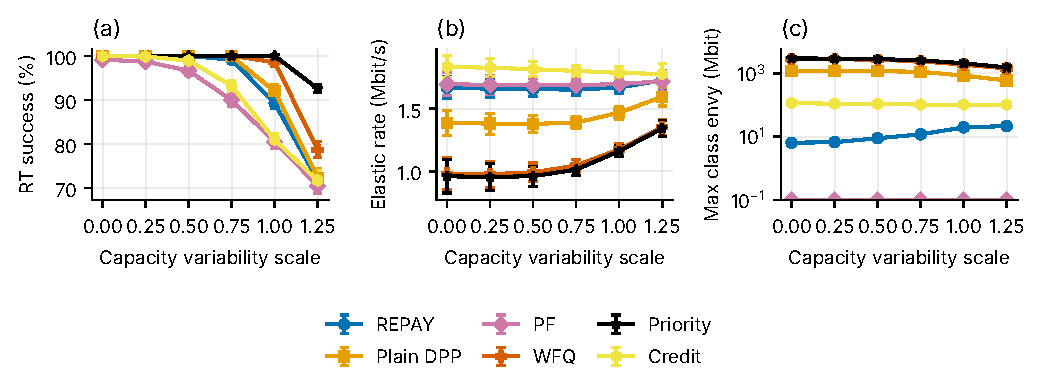
\includegraphics[width=\linewidth]{figures/fig_variability.pdf}
\caption{Effect of capacity variability (scale $0$: constant capacity; scale $1$: the default hotspot scenario) at equal mean capacity.}
\label{fig:variability}
\end{figure}

\subsection{Strategic devices}\label{sec:exp-strategic}

\paragraph{Unilateral deviations.}
We take $30$ elastic devices per trace (six traces of $3000$ slots, devices present for at least $60$ slots, $180$ devices in all) and, for each of them and each rule, re-run the whole simulation with that device declaring video for its entire stay.
This measures the exact gain, including the effect of the deviation on prices and offers that the price-taking analysis ignores.
Table~\ref{tab:deviation} and Figure~\ref{fig:deviation} report the change in the volume the device receives; since relative gains are skewed by devices that receive little when truthful, we give the median and the mean of the per-device relative gain and the pooled change in volume, with confidence intervals from a bootstrap over traces.
Under \textsc{Priority} and \textsc{WFQ} misreporting pays for more than nine devices in ten: the median device gains $170\%$ and $154\%$, and the pooled volume doubles ($+105\%$ and $+100\%$).
Under plain DPP the median gain is $77\%$ and the pooled gain $35\%$.
Under \repay{} the median change is $+1.3\%$, with a confidence interval of $[0.8,1.5]$, the mean change is $-0.1\%$, and the pooled volume falls by $10\%$.
The deviation is not harmless for everyone: $63\%$ of the devices gain something, but the gains are small (the 95th percentile is $0.09$~Mbit/s and the largest gain over a whole stay is $47$~Mbit, $4\%$ of that device's volume), and no device gains more than its bound $B_{g,\mathrm{v}}$, although the largest gain reaches $0.75$ of it, so the externality term left open after Theorem~\ref{thm:static} is not negligible here.
The picture differs by tier. Free devices, whose fair share is often below the video rate, gain a median of $2.0\%$ and $83\%$ of them gain; PAYG devices gain a median of $2.4\%$ ($67\%$ gain), although their pooled volume falls by $17\%$; premium devices lose a median of $13\%$ and only $5\%$ of them gain.
Part of the losses comes from the experiment itself: every sampled device has a link rate above $3$~Mbit/s, so declaring video caps it at $\rmax_{\mathrm{v}}$ whenever capacity is plentiful.
This is why the pooled volume also falls under \textsc{PF} and \textsc{Credit}, which ignore the declaration altogether, and the comparison that matters is between \repay{} and the rules that do use the class.

\paragraph{Short stays.}
The bound of Theorem~\ref{thm:static} is a constant per stay, so it promises little to a device that stays less than a minute.
We repeat the experiment for $120$ elastic devices with stays of $5$ to $59$ slots on four traces (Table~\ref{tab:short}).
Here misreporting does pay under \repay{} for most devices: $88\%$ of them gain and the median gain is $12\%$, although the pooled volume still falls by $4\%$ and no device gains more than $15.3$~Mbit, a quarter of its bound.
The same devices gain a median of $71\%$ under plain DPP and about $140\%$ under \textsc{Priority} and \textsc{WFQ}.
\repay{} therefore reduces the size of the gain of short-lived devices by a factor of six to eleven in the median, without reducing much the share of devices that gain ($88\%$ against $91\%$ under plain DPP).

\begin{table}[t]
\centering
\caption{Unilateral misreport by devices that stay $5$ to $59$ slots ($120$ devices on four traces).}
\label{tab:short}
\resizebox{\linewidth}{!}{% Source: results/short_stays.json; true-elastic devices with 5 to 59 slots, T=3000, seeds [0, 1, 2, 3]
\begin{tabular}{lrrrrr}
\toprule
Mechanism & n & Median rel.\ gain (\%) & Pooled volume gain (\%) & Devices gaining (\%) & Max gain (Mbit) \\
\midrule
REPAY & 120 & 10.07 & -6.04 & 82.5 & 10.403 \\
Plain DPP & 120 & 58.88 & 24.39 & 87.5 & 52.828 \\
Priority & 120 & 141.13 & 99.20 & 93.3 & 142.203 \\
WFQ & 120 & 136.37 & 92.18 & 93.3 & 138.087 \\
PF & 120 & 0.00 & -15.80 & 0.0 & 0.000 \\
\bottomrule
\end{tabular}
}
\end{table}

\paragraph{Thin markets.}
Theorem~\ref{thm:static} assumes price-taking devices, so we also compute the exact gain in markets where one device is a large part of its tier.
Tier prices are set to zero. One tier holds the potential deviator, $n_E$ other saturated elastic devices and $n_V$ genuine video flows, all present for $L$ slots, and capacity alternates between $0.3$ and $1$~Mbit/s per device.
Table~\ref{tab:thin} gives the gain of the deviator in Mbit.
It does not grow with the length of the stay: it is either a constant of about $5$~Mbit, an eighth of the bound $B_{F,\mathrm{v}}=43$~Mbit, or negative and decreasing in $L$.
With the incumbents-first rounding of an earlier version the gain in the three-device market grew linearly in $L$, which is what led us to the rotation of Section~\ref{sec:algorithm}.

\begin{table}[t]
\centering
\caption{Exact gain of one elastic device that declares video for its whole stay ($180$ devices on six traces). Relative gains are with respect to the volume under truthful declaration; brackets are 95\% bootstrap intervals over traces.}
\label{tab:deviation}
\resizebox{\linewidth}{!}{\begin{tabular}{lrrrrr}
\toprule
Mechanism & Mean gain (Mbit/s) & Median (Mbit/s) & 95th pct.\ (Mbit/s) & Gain $>0$ (\%) & Mean rel.\ gain (\%) \\
\midrule
REPAY & -0.130 & -0.008 & 0.046 & 45.0 & -3.3 \\
REPAY-E & -0.130 & -0.007 & 0.046 & 45.0 & -3.1 \\
No-debt & -0.079 & 0.003 & 0.069 & 51.7 & -2.3 \\
Plain DPP & 0.270 & 0.347 & 0.823 & 81.7 & 57.2 \\
Priority & 0.946 & 0.944 & 2.103 & 93.3 & 320.0 \\
WFQ & 0.896 & 0.883 & 2.015 & 96.7 & 271.8 \\
PF & -0.193 & -0.003 & 0.000 & 0.0 & -7.6 \\
Credit & -0.416 & -0.332 & -0.053 & 0.0 & -27.3 \\
\bottomrule
\end{tabular}
}
\end{table}

\begin{table}[t]
\centering
\caption{Thin markets: exact gain in volume (Mbit) of one elastic device that declares video for $L$ slots under \repay{}, with $n_E$ other elastic devices and $n_V$ video flows in its tier.}
\label{tab:thin}
% Source: results/thin_market.json (gain in Mbit of the deviating device)
\begin{tabular}{rrrrr}
\toprule
$n_E$ & $n_V$ & $L=500$ & $L=2000$ & $L=8000$ \\
\midrule
0 & 0 & $-75.0$ & $-300.0$ & $-1200.0$ \\
1 & 0 & $4.2$ & $4.2$ & $4.2$ \\
0 & 1 & $-8.3$ & $-45.8$ & $-195.8$ \\
1 & 1 & $-12.4$ & $-62.4$ & $-262.4$ \\
2 & 1 & $5.3$ & $5.3$ & $5.3$ \\
4 & 2 & $5.6$ & $5.6$ & $5.6$ \\
9 & 4 & $5.3$ & $5.3$ & $5.3$ \\
19 & 9 & $5.5$ & $5.5$ & $5.5$ \\
39 & 19 & $5.6$ & $5.6$ & $5.6$ \\
\bottomrule
\end{tabular}

\end{table}

\begin{figure}[t]
\centering
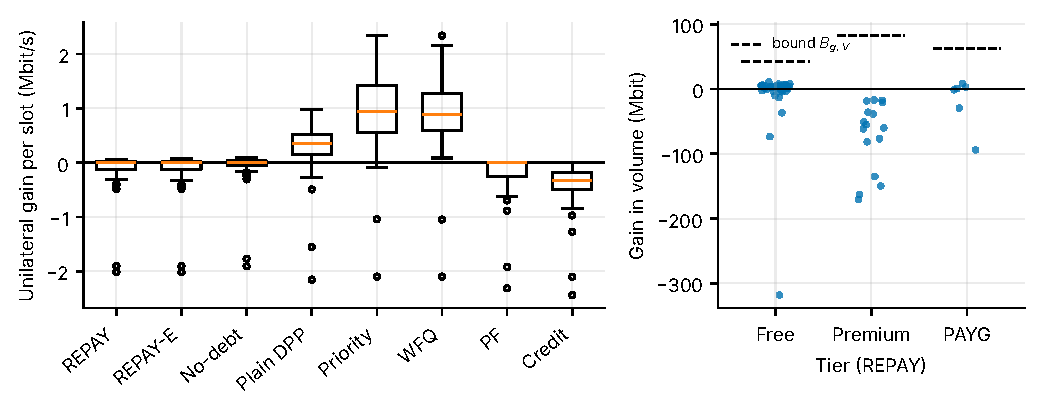
\includegraphics[width=\linewidth]{figures/fig_deviation.pdf}
\caption{Unilateral misreport. Left: gain per slot for each rule. Right: gain in volume under \repay{} compared with the bound.}
\label{fig:deviation}
\end{figure}

\paragraph{When many misreport.}
Figure~\ref{fig:collapse} lets a fraction $\rho$ of the elastic devices declare video.
Under \textsc{Priority}, \textsc{WFQ} and plain DPP a misreporting device receives more than a truthful one at every interior $\rho$ we tested ($0.25$, $0.5$, $0.75$) (for instance $1.60$ against $0.63$~Mbit/s under \textsc{Priority} at $\rho=0.25$), so $\rho$ drifts to one.
At $\rho=1$ the rules have nothing left to differentiate on. \textsc{WFQ} then serves $78\%$ of genuine RT slots, the same as \textsc{PF}, and plain DPP $88\%$, the same as \repay{}, which has no elastic device left to owe anything to; total utility falls from $72.3$ to $59.8$ under \textsc{WFQ} and from $73.2$ to $63.2$ under plain DPP.
\textsc{Priority} with admission control degrades more gracefully: it still serves $95.8\%$ of genuine RT slots at $\rho=1$, because it admits flows at the minimum rate, but calls then run at lower quality (video utility $1.75$ per slot instead of $2.53$) and every elastic device, capped at the video rate, receives $0.97$~Mbit/s.
Under \repay{} a misreporting device receives \emph{less} than a truthful one ($1.08$ against $1.23$~Mbit/s at $\rho=0.25$), so in these runs no device has a reason to leave the truthful profile $\rho=0$. Part of this sign is due to the cap of the video bundle: under class-blind \textsc{PF}, where the declaration has no other effect, misreporters receive $0.26$~Mbit/s less than truthful devices, against $0.15$ less under \repay{}. (In this paragraph the rate of an elastic device is its volume divided by the length of its stay, idle periods included, hence the lower values than in Table~\ref{tab:compare}.)
Comparing the points where each rule comes to rest, \repay{} at $\rho=0$ delivers a utility of $70.9$, an elastic rate of $1.27$~Mbit/s and a video utility of $1.92$, against $64.9$, $0.97$ and $1.75$ for \textsc{Priority} at $\rho=1$.
The two serve almost the same share of genuine RT slots ($94.7\%$ for \repay{} and $95.8\%$ for \textsc{Priority}), and \textsc{Priority} does so with an elastic rate that is $24\%$ lower.

\begin{figure}[t]
\centering
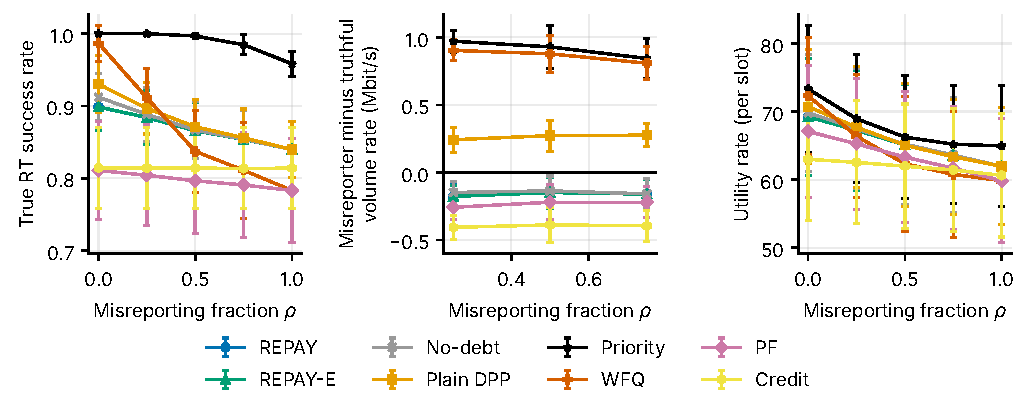
\includegraphics[width=\linewidth]{figures/fig_collapse.pdf}
\caption{A fraction $\rho$ of elastic devices declares video. Left: success of genuine RT flows. Middle: rate of misreporting minus rate of truthful elastic devices (positive values mean that misreporting pays). Right: total utility.}
\label{fig:collapse}
\end{figure}

\paragraph{The reverse deviation.}
We also let $40$ video devices declare elastic, under \repay{} and under plain DPP.
Every one of them loses utility (on average $38$ utility units over its stay under \repay{}), consistent with Proposition~\ref{prop:reverse}, which covers one slot without outstanding deficits.

\paragraph{Switching strategies.}
Finally we test dynamic declarations, on $120$ elastic devices that stay at least $200$ slots ($20$ on each of six traces).
The first attacker declares video whenever capacity is below its 40th percentile and elastic otherwise, subject to a hold-down of $\tau$ slots (Figure~\ref{fig:switching}).
Under plain DPP this strategy gains $0.18$ to $0.25$~Mbit/s for every $\tau$.
Under \repay{} it loses $0.02$ to $0.05$~Mbit/s on average, the best single device gains $0.06$~Mbit/s, and no device exceeds the bound $KB$ of Theorem~\ref{thm:dynamic}.
The second attacker is an oracle built to exploit Proposition~\ref{prop:commit}: it observes, on the truthful path, the slots in which its video reference exceeds its own allocation, and declares video exactly in those slots, again subject to a hold-down.
Under the price-taking hypothesis this strategy would gain $24$ to $40$~Mbit per device.
In the actual system it loses (Table~\ref{tab:oracle}): the mean change is between $-0.035$ and $-0.053$~Mbit/s for $\tau$ from $1$ to $60$, and at most $24\%$ of the devices gain anything, the largest gain being $0.06$~Mbit/s.
One rule of the implementation that the price-taking calculation ignores works against the attacker: a device that leaves the elastic class forfeits its deficits and restarts from zero when it returns.
Table~\ref{tab:ablation} isolates it on two of the traces. If deficits are instead kept frozen while the device poses as video, the attack becomes profitable for most devices at $\tau=1$ ($95\%$ of them gain), though by little: $0.016$~Mbit/s on average, about $1.4\%$ of their volume, and at most $0.09$~Mbit/s for any device at any $\tau$. Admitting incumbents first in addition changes nothing material.
Forfeiture is thus what makes slot-by-slot switching unprofitable in these runs (two traces; without it the mean gain is positive at $\tau=1$ and $\tau=5$ and negative at $\tau=20$). It has a cost for an honest user who makes a call and then resumes a download: the credit accumulated before the call is lost.
The experiments therefore do not show that a hold-down is needed in practice; in these experiments it is a restriction placed on the attacker, not something the allocation code enforces. Proposition~\ref{prop:commit} says that without one there is no guarantee, and we keep it as a safeguard.

\begin{figure}[t]
\centering
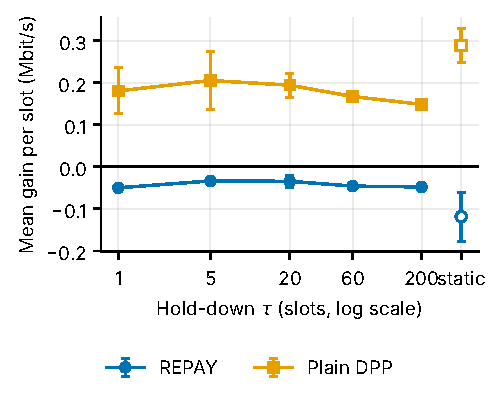
\includegraphics[width=0.45\linewidth]{figures/fig_switching.pdf}
\caption{Mean gain per slot of the congestion-triggered switching strategy as a function of the hold-down $\tau$ ($120$ devices on six traces).}
\label{fig:switching}
\end{figure}

\begin{table}[t]
\centering
\caption{Oracle slot-switching attack against \repay{} ($120$ devices on six traces): change in volume relative to truthful declaration.}
\label{tab:oracle}
\resizebox{\linewidth}{!}{% Source: results/oracle.json, scenario hotspot, six traces (seeds 0 to 5), 20 devices per trace, 120 devices in total
\begin{tabular}{rrrrrr}
\toprule
Hold-down $\tau$ & Mean gain per slot (Mbit/s) & Max gain per slot (Mbit/s) & Mean relative gain (\%) & Share with positive gain (\%) & Mean video phases \\
\midrule
1 & -0.043 & 0.040 & -4.52 & 10.0 & 64.56 \\
5 & -0.063 & 0.014 & -5.96 & 1.7 & 23.18 \\
20 & -0.055 & 0.019 & -4.30 & 4.2 & 8.30 \\
60 & -0.062 & 0.043 & -3.68 & 15.8 & 3.42 \\
\bottomrule
\end{tabular}
}
\end{table}

\begin{table}[t]
\centering
\caption{Oracle attack ($40$ devices on two traces) against \repay{}, against a variant in which deficits are kept frozen while a device declares video, and against that variant with incumbents-first admission.}
\label{tab:ablation}
\resizebox{\linewidth}{!}{% Source: results/oracle_ablation.json, scenario hotspot, seeds 0 and 1, 20 devices per seed
\begin{tabular}{llrrr}
\toprule
Rule & Hold-down $\tau$ & Mean gain per slot (Mbit/s) & Max gain per slot (Mbit/s) & Share gaining (\%) \\
\midrule
REPAY & 1 & -0.048 & 0.017 & 5.0 \\
REPAY & 5 & -0.069 & -0.003 & 0.0 \\
REPAY & 20 & -0.059 & 0.019 & 5.0 \\
\midrule
REPAY-keep & 1 & 0.011 & 0.048 & 85.0 \\
REPAY-keep & 5 & -0.012 & 0.061 & 60.0 \\
REPAY-keep & 20 & -0.024 & 0.116 & 60.0 \\
\midrule
REPAY-keep-sticky & 1 & 0.008 & 0.049 & 77.5 \\
REPAY-keep-sticky & 5 & -0.014 & 0.058 & 47.5 \\
REPAY-keep-sticky & 20 & -0.027 & 0.087 & 55.0 \\
\bottomrule
\end{tabular}
}
\end{table}

\subsection{Traffic mix and population size}\label{sec:exp-mix}

The comparisons so far use one traffic mix, in which $35\%$ of the devices are real-time, and about $75$ devices.
We vary both on the hotspot scenario with truthful devices.
First, the real-time share $\rho_{\mathrm{RT}}$ takes the values $5$, $10$, $20$, $35$ and $50\%$, split between video and gaming in the ratio $5:2$ of the default (five traces per value).
Second, at the default mix, the arrival rate, the batch size and the mean capacity are multiplied together by $0.25$, $0.5$, $1$, $2$ and $4$, so that the load per device is unchanged and between $19$ and $288$ devices are present on average (three traces per value).
Third, at $\rho_{\mathrm{RT}}=10\%$ we repeat the unilateral deviation of Section~\ref{sec:exp-strategic} for $60$ elastic devices on two traces.

Figure~\ref{fig:mix} shows the first sweep.
\repay{} serves between $91.1\%$ and $95.1\%$ of RT slots at every share, with class envy between $5$ and $18$~Mbit and an elastic rate between $1.65$ and $1.72$~Mbit/s, close to that of \textsc{PF} ($1.67$ to $1.79$).
\textsc{Priority} serves all RT slots at every share, with class envy above $2000$~Mbit; plain DPP serves at least $99.4\%$ with class envy above $1000$~Mbit.
Capped priority with $q=0.3$ changes character with the mix: when real-time devices are few the cap does not bind, and it behaves like strict priority ($100\%$ of RT slots, class envy of $2070$~Mbit at $\rho_{\mathrm{RT}}=5\%$), and when they are many it rations them ($86.7\%$ of RT slots at $\rho_{\mathrm{RT}}=50\%$, with an elastic rate of $2.32$~Mbit/s).
Table~\ref{tab:mix-dev} gives the corresponding incentives at $\rho_{\mathrm{RT}}=10\%$: under capped priority the median misreporting device gains $113\%$ and $82\%$ of the devices gain, close to \textsc{WFQ} ($133\%$) and \textsc{Priority} ($145\%$), while under \repay{} the median change is $-0.9\%$, $45\%$ of the devices gain and none exceeds its bound (the largest gain is $0.19$ of it).
Without the debt price the median gain is $3.4\%$, $75\%$ of the devices gain and three of the $60$ exceed the bound, by up to a factor $1.75$.

The population sweep (Table~\ref{tab:mix-scale}) shows no degradation with size: \repay{} serves between $92.9\%$ and $95.5\%$ of RT slots from $19$ to $288$ devices, its class envy decreases from $19$ to $13$~Mbit, and its elastic rate stays within $0.06$~Mbit/s of that of \textsc{PF}.
This is the experiment in which the unnormalised tier queues of the earlier version failed (Section~\ref{sec:algorithm}).

\begin{figure}[t]
\centering
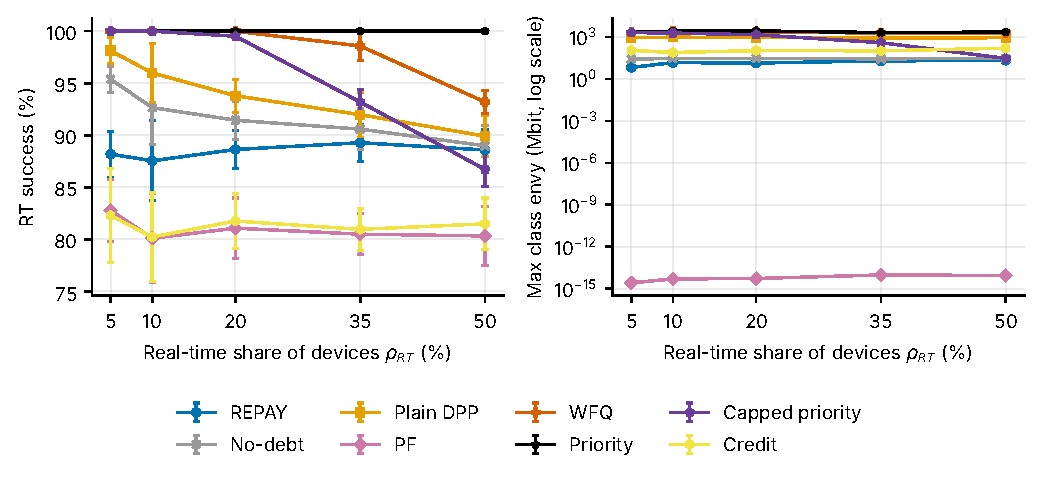
\includegraphics[width=\linewidth]{figures/fig_mix.pdf}
\caption{Hotspot scenario with truthful devices, varying the share of real-time devices (mean over five traces): (a) RT success, (b) maximum class envy (logarithmic scale; \textsc{PF} has none).}
\label{fig:mix}
\end{figure}

\begin{table}[t]
\centering
\caption{RT success (\%) when the population is scaled at the default mix (columns: mean number of devices present; mean over three traces $\pm$ half-width of the 95\% interval).}
\label{tab:mix-scale}
\resizebox{\linewidth}{!}{% Source: results/mix.json, part 2; hotspot default mix, truthful devices, T=6000, seeds 0 to 2; columns: mean number of active devices; cells: RT success (\%) mean $\pm$ 95% CI half-width
\begin{tabular}{lrrrrr}
\toprule
Mechanism & 19 & 37 & 75 & 146 & 288 \\
\midrule
REPAY & 88.3 $\pm$ 4.2 & 89.9 $\pm$ 3.2 & 88.6 $\pm$ 2.4 & 88.4 $\pm$ 2.7 & 69.5 $\pm$ 2.0 \\
No-debt & 89.6 $\pm$ 3.7 & 91.4 $\pm$ 2.7 & 89.6 $\pm$ 1.4 & 89.4 $\pm$ 2.4 & 71.5 $\pm$ 1.0 \\
Plain DPP & 90.4 $\pm$ 3.3 & 93.0 $\pm$ 1.6 & 90.8 $\pm$ 0.2 & 91.3 $\pm$ 1.8 & 73.4 $\pm$ 2.9 \\
PF & 81.2 $\pm$ 8.1 & 80.1 $\pm$ 8.2 & 81.1 $\pm$ 4.5 & 82.4 $\pm$ 4.3 & 82.2 $\pm$ 3.3 \\
WFQ & 96.5 $\pm$ 3.1 & 97.3 $\pm$ 2.4 & 98.2 $\pm$ 3.4 & 99.5 $\pm$ 0.4 & 99.7 $\pm$ 0.1 \\
Priority & 100.0 $\pm$ 0.0 & 100.0 $\pm$ 0.0 & 100.0 $\pm$ 0.0 & 100.0 $\pm$ 0.0 & 100.0 $\pm$ 0.0 \\
Capped priority & 90.9 $\pm$ 2.1 & 91.9 $\pm$ 3.2 & 92.8 $\pm$ 2.0 & 94.7 $\pm$ 0.7 & 95.1 $\pm$ 1.1 \\
Credit & 81.8 $\pm$ 3.9 & 80.6 $\pm$ 7.2 & 81.4 $\pm$ 5.0 & 83.0 $\pm$ 3.8 & 83.1 $\pm$ 4.1 \\
\bottomrule
\end{tabular}
}
\end{table}

\begin{table}[t]
\centering
\caption{Unilateral misreport at a real-time share of $10\%$ ($60$ devices on two traces). The bound is $B_{g,\mathrm{v}}$ at $V=20$ for the tier of the device; capped priority uses $q=0.3$.}
\label{tab:mix-dev}
\resizebox{\linewidth}{!}{% Source: results/mix.json, part 3; rho_RT=0.1, T=3000, seeds [0, 1], 30 true-elastic devices per seed; devices above bound counts gains above $B_{g,1}$ (REPAY and no-debt only)
\begin{tabular}{lrrrrr}
\toprule
Mechanism & $n$ & Median rel.\ gain (\%) & Pooled volume gain (\%) & Devices gaining (\%) & Devices above bound \\
\midrule
REPAY & 60 & -0.90 & -13.31 & 45.0 & 0 \\
No-debt & 60 & 3.37 & -5.06 & 75.0 & 3 \\
Plain DPP & 60 & 72.71 & 28.11 & 81.7 & -- \\
Priority & 60 & 144.79 & 79.78 & 90.0 & -- \\
WFQ & 60 & 133.21 & 75.17 & 90.0 & -- \\
Capped priority & 60 & 113.34 & 51.11 & 81.7 & -- \\
PF & 60 & -0.11 & -15.64 & 0.0 & -- \\
\bottomrule
\end{tabular}
}
\end{table}

\subsection{Trace-driven evaluation}\label{sec:exp-real}

The experiments so far use synthetic arrivals, stays, demands, classes and capacity.
We now build them from public logs. The result is a trace-driven scenario, not the trace of one operator.

\paragraph{Construction.}
Arrivals, stays, demand levels and service classes come from the session logs that the City of Paris publishes for its public Wi-Fi network \citep{pariswifi2026}, which give, for every session, its start, its duration and the bytes and packets transferred in each direction.
We take a site with a large population (code PW0127, ``Quartier Jeunes'' in the data), the six days with the most sessions since January 2025 and, in each, the two hours with the highest occupancy; a second, smaller site (PW0232, the Petit Palais museum) serves as a check.
These are the busiest days by construction and all six are Thursdays, four of them consecutive, so the traces are not an independent sample of days.
A device is a session: the network limits connections to two hours, so a user who reconnects counts as a new device, and the roughly one hundred sessions already open at the start of a window enter with zero deficits and are observed only for the part of their stay that falls in the window.

The \emph{class} of a device is inferred from the traffic of its session.
A session is taken to be a video call if its traffic is two-way, with a ratio of uplink to downlink bytes between $1/3$ and $3$, and its mean uplink rate is at least $0.1$~Mbit/s; to be a game if it is two-way at a lower uplink rate (at least $0.01$~Mbit/s) with a mean downlink packet below $700$ bytes; and to be elastic otherwise.
This is a heuristic on session averages and not a validated classifier, so we also report a stricter rule (ratio between $1/2$ and $2$ for both classes, uplink at least $0.2$~Mbit/s for video).
Only the class is taken from the log: a device classified as real-time has the rate requirements of the model ($\rmin_{\mathrm{v}}$, $\rmax_{\mathrm{v}}$, $r_{\mathrm{g}}$), not its logged rate.
Table~\ref{tab:real-classes} gives the resulting shares: $8\%$ of the sessions of the main site are video-like and $2\%$ game-like, against the $25\%$ and $10\%$ that we assumed in the synthetic hotspot.
For an elastic device the demand cap is set so that its mean demand equals the mean downlink rate observed for its session (median cap $0.29$ to $0.52$~Mbit/s), with on--off periods as before.

The logs contain no \emph{tier}, since the network is free.
We draw tiers at random from an estimate assembled from two public figures: the connectivity sessions of a commercial in-flight Wi-Fi service equalled $11.6\%$ of its passengers in North America in 2018, sessions paid by third parties or airlines included \citep{gogo2019tenk}, which we take as a proxy for the share of paying users, and $8\%$ of mobile users in metropolitan France are on prepaid cards \citep{arcep2026mobile}, which we take as the share of pay-as-you-go among paying users.
This gives $88.4\%$ free, $10.7\%$ premium and $0.9\%$ PAYG. It is a rough estimate from unrelated markets; a variant with every device in the free tier is reported as well.

\emph{Capacity} follows the throughput logs, at roughly one sample per second, that \citet{riiser2013commute} recorded in a 3G network on metro, tram, train, bus and ferry routes in Oslo, which has nothing to do with the Paris network; we treat each sample as one slot (gaps in the logs are skipped), concatenate the logs in random order and scale them by a constant so that mean capacity is a multiple (the \emph{load}, $1$ by default) of the mean nominal demand.
Table~\ref{tab:real-traces} describes the traces.
Compared with the synthetic hotspot, about $120$ devices are present instead of $75$, the median stay in the window is $35$ to $48$ minutes instead of a mean of four minutes, real-time traffic is three times rarer, elastic demand is light, and capacity is far more variable, with a coefficient of variation of $0.70$ to $0.84$ and deep fades.
All parameters of the rules, including $V=20$ and the cap $q=0.3$, are those of the synthetic experiments and were not retuned.

\begin{table}[t]
\centering
\caption{Share of sessions classified as video-like and game-like, and median session rates of each group (sessions since January 2025).}
\label{tab:real-classes}
\resizebox{0.85\linewidth}{!}{% Source: results/real_compare.json, class_shares (experiments/data_real.py): sessions of duration >= 5 s starting on or after 2025-01-01; medians of session-average rates.
\begin{tabular}{llrrrrr}
\toprule
Site & Rule & Share video (\%) & Share gaming (\%) & Video down (Mbit/s) & Video up (Mbit/s) & Gaming down (Mbit/s) \\
\midrule
PW0127 & default & 7.7 & 2.4 & 0.353 & 0.241 & 0.047 \\
PW0127 & strict & 3.0 & 2.3 & 0.515 & 0.460 & 0.056 \\
PW0232 & default & 12.0 & 0.5 & 0.349 & 0.322 & 0.029 \\
PW0232 & strict & 5.5 & 0.4 & 0.478 & 0.476 & 0.040 \\
\bottomrule
\end{tabular}
}
\end{table}

\begin{table}[t]
\centering
\caption{Trace-driven scenario: two-hour windows of the Paris public Wi-Fi session logs, with capacity from 3G commute logs scaled to load $1$.}
\label{tab:real-traces}
\resizebox{\linewidth}{!}{% Source: results/real_compare.json (experiments/data_real.py); PW0127 windows, and PW0232 averaged over its six windows.
\begin{tabular}{lllrrrrrr}
\toprule
Trace & Date & Devices & Mean conc. & Median stay (s) & Median elastic cap (Mbit/s) & 90th pct.\ elastic cap (Mbit/s) & Mean capacity (Mbit/s) & CV of capacity \\
\midrule
PW0127, $k=0$ & 2025-04-03 & 283 & 125.5 & 2677 & 0.28 & 1.39 & 66.2 & 0.72 \\
PW0127, $k=1$ & 2025-10-30 & 270 & 120.6 & 2645 & 0.39 & 1.33 & 91.1 & 0.84 \\
PW0127, $k=2$ & 2026-04-09 & 305 & 131.7 & 2535 & 0.43 & 1.45 & 96.7 & 0.74 \\
PW0127, $k=3$ & 2026-04-16 & 226 & 88.1 & 2078 & 0.64 & 1.82 & 68.1 & 0.70 \\
PW0127, $k=4$ & 2026-04-23 & 272 & 113.2 & 2407 & 0.33 & 1.68 & 81.5 & 0.75 \\
PW0127, $k=5$ & 2026-04-30 & 295 & 131.4 & 2880 & 0.42 & 1.66 & 95.4 & 0.70 \\
\midrule
PW0232, mean of $k=0,\dots,5$ & -- & 153.7 & 37.3 & 1288 & 0.59 & 1.93 & 28.3 & 0.74 \\
\bottomrule
\end{tabular}
}
\end{table}

\begin{table}[t]
\centering
\caption{Trace-driven scenario, site PW0127, load $1$, truthful devices (mean over six traces $\pm$ half-width of the 95\% interval). The premium target is $0.8$.}
\label{tab:real-compare}
\resizebox{\linewidth}{!}{% Source: results/real_compare.json, variant main (experiments/exp_real.py); site PW0127, load 1.0; mean $\pm$ 95% Student-t half-width over six traces.
\begin{tabular}{lrrrrrr}
\toprule
Mechanism & Utility & RT success (\%) & Video success (\%) & Elastic rate (Mbit/s) & Max class envy (Mbit) & Premium served ratio \\
\midrule
REPAY & 44.73 $\pm$ 7.04 & 82.0 $\pm$ 4.4 & 78.8 $\pm$ 3.7 & 0.44 $\pm$ 0.08 & 42.33 $\pm$ 12.98 & 1.03 $\pm$ 0.10 \\
No-debt & 45.02 $\pm$ 7.11 & 88.5 $\pm$ 3.2 & 86.2 $\pm$ 3.0 & 0.44 $\pm$ 0.08 & 43.22 $\pm$ 10.13 & 0.97 $\pm$ 0.08 \\
Plain DPP & 46.18 $\pm$ 7.20 & 93.9 $\pm$ 2.8 & 93.2 $\pm$ 2.7 & 0.40 $\pm$ 0.08 & 2460.87 $\pm$ 289.67 & 1.07 $\pm$ 0.12 \\
PF & 43.47 $\pm$ 6.87 & 75.4 $\pm$ 4.9 & 73.2 $\pm$ 4.6 & 0.44 $\pm$ 0.08 & 0.00 $\pm$ 0.00 & 1.04 $\pm$ 0.08 \\
WFQ & 44.80 $\pm$ 6.97 & 94.1 $\pm$ 1.6 & 93.6 $\pm$ 1.6 & 0.32 $\pm$ 0.07 & 5088.25 $\pm$ 1132.22 & 0.99 $\pm$ 0.20 \\
Priority & 45.13 $\pm$ 7.11 & 97.1 $\pm$ 1.2 & 96.6 $\pm$ 1.4 & 0.32 $\pm$ 0.07 & 5356.58 $\pm$ 1313.04 & 0.91 $\pm$ 0.19 \\
Capped priority ($q=0.3$) & 45.24 $\pm$ 7.01 & 91.3 $\pm$ 2.1 & 89.8 $\pm$ 2.3 & 0.43 $\pm$ 0.07 & 1159.08 $\pm$ 443.83 & 0.92 $\pm$ 0.04 \\
Credit & 40.36 $\pm$ 6.41 & 58.8 $\pm$ 6.5 & 50.2 $\pm$ 4.4 & 0.47 $\pm$ 0.08 & 167.45 $\pm$ 163.49 & 0.87 $\pm$ 0.06 \\
\bottomrule
\end{tabular}
}
\end{table}

\begin{table}[t]
\centering
\caption{Trace-driven scenario, site PW0127: RT success and elastic rate at three loads (mean over six traces).}
\label{tab:real-load}
% Source: results/real_compare.json (experiments/exp_real.py); site PW0127, means over six traces.
\begin{tabular}{lrrrrrr}
\toprule
 & \multicolumn{3}{c}{RT success (\%)} & \multicolumn{3}{c}{Elastic rate (Mbit/s)} \\
\cmidrule(lr){2-4}\cmidrule(lr){5-7}
Mechanism & 0.7 & 1.0 & 1.5 & 0.7 & 1.0 & 1.5 \\
\midrule
REPAY & 71.4 & 81.5 & 88.2 & 0.35 & 0.42 & 0.49 \\
No-debt & 74.8 & 84.1 & 89.9 & 0.35 & 0.43 & 0.49 \\
Plain DPP & 78.9 & 86.4 & 91.2 & 0.24 & 0.33 & 0.43 \\
PF & 64.2 & 75.8 & 84.1 & 0.37 & 0.43 & 0.50 \\
WFQ & 80.3 & 86.1 & 90.4 & 0.09 & 0.19 & 0.32 \\
Priority & 91.6 & 94.0 & 95.9 & 0.07 & 0.16 & 0.30 \\
Capped priority ($q=0.3$) & 72.6 & 81.1 & 87.3 & 0.48 & 0.52 & 0.56 \\
Credit & 53.1 & 66.3 & 77.8 & 0.43 & 0.49 & 0.54 \\
\bottomrule
\end{tabular}

\end{table}

\begin{table}[t]
\centering
\caption{Trace-driven scenario, site PW0127, load $1$: sensitivity to the classification rule and to the tier assumption.}
\label{tab:real-variants}
\resizebox{\linewidth}{!}{% Source: results/real_compare.json (experiments/exp_real.py); site PW0127, load 1.0; mean $\pm$ 95% Student-t half-width over six traces. Strict rule: sym in [0.5, 2], up_min 0.2. All free: every device in the free tier (as in the logged network).
\begin{tabular}{lrrrrrr}
\toprule
 & \multicolumn{3}{c}{strict rule} & \multicolumn{3}{c}{all devices free} \\
\cmidrule(lr){2-4}\cmidrule(lr){5-7}
Mechanism & RT success (\%) & Elastic rate (Mbit/s) & Max class envy (Mbit) & RT success (\%) & Elastic rate (Mbit/s) & Max class envy (Mbit) \\
\midrule
REPAY & 87.3 $\pm$ 2.9 & 0.44 $\pm$ 0.08 & 15.29 $\pm$ 3.81 & 83.7 $\pm$ 3.6 & 0.45 $\pm$ 0.07 & 56.00 $\pm$ 14.80 \\
No-debt & 94.2 $\pm$ 1.7 & 0.44 $\pm$ 0.08 & 45.70 $\pm$ 15.10 & 90.4 $\pm$ 2.6 & 0.45 $\pm$ 0.07 & 34.84 $\pm$ 3.65 \\
Plain DPP & 98.4 $\pm$ 1.2 & 0.42 $\pm$ 0.08 & 2299.79 $\pm$ 431.29 & 97.1 $\pm$ 1.2 & 0.40 $\pm$ 0.07 & 2664.79 $\pm$ 233.44 \\
PF & 79.8 $\pm$ 5.4 & 0.44 $\pm$ 0.08 & 0.00 $\pm$ 0.00 & 76.1 $\pm$ 4.2 & 0.45 $\pm$ 0.07 & 0.00 $\pm$ 0.00 \\
WFQ & 97.3 $\pm$ 2.0 & 0.40 $\pm$ 0.08 & 4226.98 $\pm$ 907.16 & 95.0 $\pm$ 2.0 & 0.32 $\pm$ 0.07 & 5367.10 $\pm$ 1073.94 \\
Priority & 98.6 $\pm$ 1.0 & 0.40 $\pm$ 0.08 & 4433.03 $\pm$ 915.53 & 97.1 $\pm$ 1.2 & 0.32 $\pm$ 0.07 & 5363.43 $\pm$ 1073.40 \\
Capped priority ($q=0.3$) & 95.6 $\pm$ 2.2 & 0.42 $\pm$ 0.08 & 3194.39 $\pm$ 363.56 & 91.5 $\pm$ 2.2 & 0.43 $\pm$ 0.07 & 991.82 $\pm$ 365.81 \\
Credit & 71.4 $\pm$ 4.5 & 0.45 $\pm$ 0.08 & 284.40 $\pm$ 161.43 & 59.0 $\pm$ 5.3 & 0.47 $\pm$ 0.07 & 149.32 $\pm$ 150.79 \\
\bottomrule
\end{tabular}
}
\end{table}

\begin{table}[t]
\centering
\caption{Trace-driven scenario, site PW0127, load $1$: one elastic device declares video for its whole stay ($120$ devices on six traces).}
\label{tab:real-dev}
\resizebox{0.9\linewidth}{!}{% Source: results/real_deviation.json, variant main (experiments/exp_real.py); site PW0127, load 1.0, six traces, 20 true-elastic devices per trace.
\begin{tabular}{lrrrrr}
\toprule
Mechanism & $n$ & Median rel.\ gain (\%) & Pooled volume gain (\%) & Devices gaining (\%) & 95th pct.\ gain (Mbit/s) \\
\midrule
REPAY & 120 & -0.36 & -0.66 & 47.5 & 0.0390 \\
Plain DPP & 120 & 27.69 & 36.60 & 100.0 & 0.4121 \\
Priority & 120 & 64.28 & 83.22 & 100.0 & 0.7362 \\
WFQ & 120 & 65.99 & 78.74 & 100.0 & 0.7270 \\
PF & 120 & 0.00 & -0.78 & 0.0 & 0.0000 \\
Capped priority ($q=0.3$) & 120 & 3.65 & 9.40 & 65.8 & 0.1815 \\
\bottomrule
\end{tabular}
}
\end{table}

\paragraph{Truthful devices.}
Table~\ref{tab:real-compare} repeats the comparison of Section~\ref{sec:exp-compare}.
\repay{} serves $82.4\%$ of RT slots against $75.4\%$ for \textsc{PF}; the paired difference over the six traces is $7.0\pm0.9$ points, at an elastic rate lower by $0.004\pm0.001$~Mbit/s.
Its class envy is $44$~Mbit on average and at most $69$~Mbit, and no deficit exceeds $0.39$ of its bound in any run.
The rules that give RT flows priority serve many more RT slots than \repay{} here, whereas on the synthetic hotspot the difference was at most five points: plain DPP serves $13.8\pm3.1$ points more RT slots than \repay{}, \textsc{WFQ} $11.7\pm3.3$ and \textsc{Priority} $14.7\pm3.8$, while the elastic rate falls by $0.05$ to $0.12$~Mbit/s, that is by $11\%$ under plain DPP and $27$--$28\%$ under \textsc{WFQ} and \textsc{Priority}.
The reason is the traffic mix. When one device in ten is real-time, serving all of them first costs the other nine less on average than in the synthetic hotspot, and the cost is concentrated: class envy under these rules is $2600$ to $5400$~Mbit.
Capped priority with the untuned cap $q=0.3$ sits in between, with $8.9\pm3.0$ points more RT slots than \repay{} at an elastic rate that does not differ significantly ($-0.007\pm0.014$~Mbit/s) and class envy of $1160$~Mbit.
The variant without the debt price serves $7.6\pm1.8$ points more RT slots than \repay{} at the same elastic rate and with about the same class envy ($46$~Mbit).
The premium service level is met on average by every rule; \textsc{Priority} falls below the target on two of the six traces, and \textsc{WFQ} and \textsc{Credit} on one each.
The pattern is the same at loads $0.7$ and $1.5$ (Table~\ref{tab:real-load}), on the second site ($82.9\%$ for \repay{} against $76.7\%$ for \textsc{PF} and $94.1\%$ for plain DPP), under the stricter classification rule and with all devices free (Table~\ref{tab:real-variants}).

\paragraph{The role of $V$ and of the debt price.}
On these traces \repay{} gives up twelve to fifteen points of RT success relative to the priority rules, and one may ask whether a larger $V$, which loosens the envy bound, would recover them.
It does not (Table~\ref{tab:real-sweep} and Figure~\ref{fig:real-frontier}).
Between $V=5$ and $V=500$ the RT success of \repay{} rises only from $81.3\%$ to $86.9\%$, while its class envy grows from $24$ to $189$~Mbit; plain DPP stays between $95\%$ and $97\%$ over the same range.
What holds \repay{} back is the debt price, the part of the deficit that is charged to the RT group.
The variant without it (No-debt), which keeps the deficit queues and the bonus of the creditor, serves $88.0\%$ of RT slots at $V=5$ with a class envy of $19$~Mbit and $96.6\%$ at $V=500$ with $467$~Mbit: for a given level of envy it serves about seven points more RT slots than \repay{}, at the same elastic rate, and its deficits also stay below their bound (at most $0.82$ of it in any run).
Capped priority traces a similar curve when its cap is varied ($87.4\%$ at $q=0.2$ with envy of $239$~Mbit), with no bound behind it.
At equal $V$ the debt price does reduce the gain from misreporting, as the next paragraph shows, but $V$ and the debt price turn out to be substitutes for that purpose, and the cheaper instrument is a small $V$.
The variant without the debt price at $V=5$ serves $88.0\%$ of RT slots with a class envy of $19$~Mbit and leaves a median gain from misreporting of $-0.2\%$ ($45\%$ of the devices gain, three exceed the bound); the full rule at $V=20$ serves $82.4\%$ with $44$~Mbit and $-0.4\%$ ($48\%$ gain, nine exceed the bound).
On these traces the first configuration is therefore the better one on RT success and envy, at a similar incentive to misreport.
We had taken the full rule with $V=20$ as the default on the strength of the synthetic experiments, where No-debt at the same $V$ served $2.6$ more points of RT slots at a higher envy ($25$ against $15$~Mbit), and did not retune it; the traces show that this default is not the best one when real-time traffic is rare.

\begin{figure}[t]
\centering
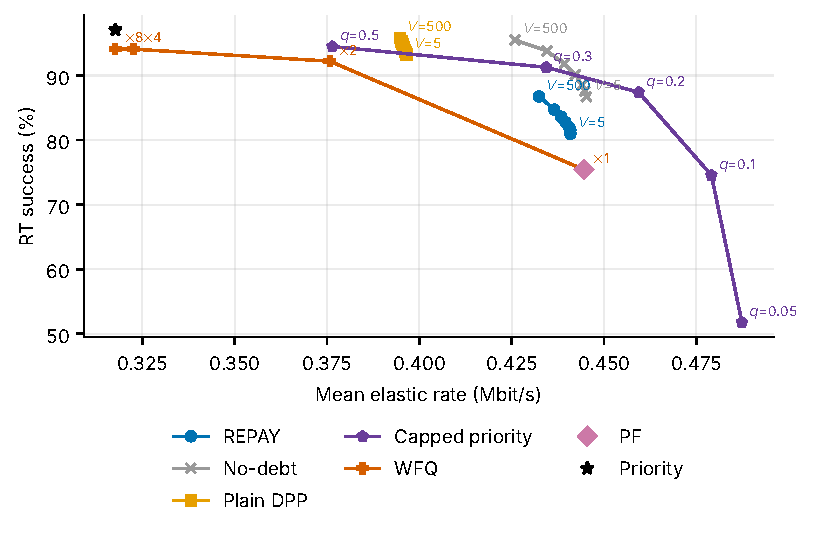
\includegraphics[width=0.75\linewidth]{figures/fig_real_frontier.pdf}
\caption{Trace-driven scenario, site PW0127, load $1$: RT success against elastic rate when the parameter of each rule is varied (mean over six traces). For the families swept over $V$ only the smallest and the largest value are labelled.}
\label{fig:real-frontier}
\end{figure}

\begin{table}[t]
\centering
\caption{Trace-driven scenario: effect of $V$ (mean over six traces). The class envy reported is the largest over tiers and RT classes; the bound shown is that of the free tier and the video class, and the bounds of the premium tier and of the gaming class are larger.}
\label{tab:real-sweep}
\resizebox{0.9\linewidth}{!}{% Source: results/real_sweep.json, variant main (experiments/exp_real_sweep.py); site PW0127, load 1.0; means over 6 traces. Envy bound: Params(V).B(0, 1), free tier, video; -- for Plain DPP, which keeps no deficits.
\begin{tabular}{llrrrrr}
\toprule
Mechanism & $V$ & RT success (\%) & Elastic rate (Mbit/s) & Max class envy (Mbit) & Envy bound $B$ (Mbit) & Premium served ratio \\
\midrule
REPAY & 5 & 81.3 & 0.44 & 24.12 & 13.0 & 1.025 \\
REPAY & 10 & 81.9 & 0.44 & 35.48 & 23.0 & 1.022 \\
REPAY & 20 & 82.4 & 0.44 & 43.92 & 43.0 & 1.020 \\
REPAY & 50 & 83.2 & 0.44 & 53.65 & 103.0 & 1.018 \\
REPAY & 100 & 84.1 & 0.44 & 69.43 & 203.0 & 1.019 \\
REPAY & 200 & 85.0 & 0.44 & 99.73 & 403.0 & 1.021 \\
REPAY & 500 & 86.9 & 0.43 & 189.25 & 1003.0 & 1.025 \\
\midrule
No-debt & 5 & 88.0 & 0.45 & 18.64 & 13.0 & 0.936 \\
No-debt & 10 & 89.1 & 0.45 & 30.57 & 23.0 & 0.928 \\
No-debt & 20 & 90.0 & 0.44 & 46.12 & 43.0 & 0.921 \\
No-debt & 50 & 91.6 & 0.44 & 77.26 & 103.0 & 0.910 \\
No-debt & 100 & 93.2 & 0.44 & 122.87 & 203.0 & 0.904 \\
No-debt & 200 & 95.2 & 0.43 & 234.89 & 403.0 & 0.908 \\
No-debt & 500 & 96.6 & 0.43 & 467.00 & 1003.0 & 0.937 \\
\midrule
Plain DPP & 5 & 95.5 & 0.39 & 2525.02 & -- & 1.049 \\
Plain DPP & 10 & 95.9 & 0.39 & 2542.32 & -- & 1.044 \\
Plain DPP & 20 & 96.2 & 0.39 & 2556.78 & -- & 1.039 \\
Plain DPP & 50 & 96.5 & 0.39 & 2570.50 & -- & 1.033 \\
Plain DPP & 100 & 96.7 & 0.39 & 2576.73 & -- & 1.030 \\
Plain DPP & 200 & 96.8 & 0.39 & 2580.46 & -- & 1.029 \\
Plain DPP & 500 & 96.8 & 0.39 & 2582.72 & -- & 1.027 \\
\bottomrule
\end{tabular}
}
\end{table}

\begin{table}[t]
\centering
\caption{Trace-driven scenario: unilateral misreport under \repay{} and under the variant without the debt price, for several $V$ ($120$ devices on six traces). The bound is $B_{g,\mathrm{v}}$ at that $V$ for the tier of the device.}
\label{tab:real-sweep-dev}
\resizebox{0.9\linewidth}{!}{% Source: results/real_sweep.json and results/real_deviation.json (reference row); variant main, site PW0127, load 1.0, six traces, 20 true-elastic devices per trace. Bound: Params(V).B(tier, 1) of the device's tier.
\begin{tabular}{lrrrrrr}
\toprule
Rule & $V$ & Median rel.\ gain (\%) & Pooled volume gain (\%) & Devices gaining (\%) & Devices above bound & Max gain / bound \\
\midrule
REPAY (ref.) & 20 & -0.36 & -0.66 & 47.5 & 9 & 11.638 \\
\midrule
REPAY & 5 & -1.38 & -1.46 & 37.5 & 13 & 36.091 \\
REPAY & 50 & 0.68 & 0.20 & 55.8 & 1 & 5.046 \\
REPAY & 100 & 1.34 & 1.29 & 63.3 & 1 & 2.668 \\
REPAY & 200 & 2.76 & 3.11 & 75.0 & 1 & 1.473 \\
\midrule
No-debt & 5 & -0.15 & -1.02 & 45.0 & 3 & 17.762 \\
No-debt & 20 & 1.92 & 1.25 & 85.0 & 2 & 7.725 \\
No-debt & 50 & 6.86 & 3.99 & 94.2 & 2 & 4.375 \\
No-debt & 100 & 11.59 & 7.23 & 99.2 & 2 & 2.889 \\
No-debt & 200 & 20.31 & 12.02 & 100.0 & 1 & 1.794 \\
\bottomrule
\end{tabular}
}
\end{table}

\paragraph{Misreporting.}
Table~\ref{tab:real-dev} repeats the unilateral deviation of Section~\ref{sec:exp-strategic} for $20$ elastic devices per trace.
Under \textsc{Priority} and \textsc{WFQ} every device gains, with a median gain of about $65\%$; under plain DPP every device gains and the median gain is $28\%$; under capped priority $66\%$ of the devices gain, with a median of $3.7\%$.
Under \repay{} the median change is $-0.4\%$, the pooled change $-0.7\%$, and $48\%$ of the sampled devices gain something from this one deviation.

The bound of Theorem~\ref{thm:static} is exceeded, however, by $9$ of the $120$ devices.
Eight of them are in the free tier and gain between $1.07$ and $1.82$ times $B_{F,\mathrm{v}}$, that is $46$ to $78$~Mbit or $2.5$ to $13\%$ of their volume, over stays of twenty minutes to two hours in the window.
The ninth is a premium device that gains $966$~Mbit, almost twelve times its bound and $16\%$ of its volume.
The premium tier of that trace has $25$ devices and two video flows, so the device is often the only video flow of its tier and its reference on the truthful path is zero: this is the empty-group case in which the price-taking hypothesis fails outright (Section~\ref{sec:ic}).
With the entrant offer of \textsc{Repay-E} the same device gains $222$~Mbit, still more than twice its bound.
Table~\ref{tab:real-sweep-dev} shows how these gains move with $V$ and what the debt price contributes.
Under \repay{} the median gain rises from $-1.4\%$ at $V=5$ and $-0.4\%$ at $V=20$ to $2.8\%$ at $V=200$, and the share of devices that gain from $38\%$ to $75\%$.
Without the debt price the gain is larger at every $V$: the median is $-0.2\%$ at $V=5$ ($45\%$ of the devices gain), $1.9\%$ at $V=20$ ($85\%$) and $20\%$ at $V=200$, where every device gains and the figure approaches the $28\%$ of plain DPP.
The number of devices above the bound moves the other way, because the bound shrinks with $V$: thirteen under \repay{} and three without the debt price at $V=5$, and one or two for $V\ge50$.
None of this contradicts the theorem, whose hypothesis is not satisfied, and every deficit stays below its bound as Theorem~\ref{thm:bound} requires; but it shows that in thin tiers and over long stays the incentive guarantee is weaker than the bound suggests, and that the gains, although small relative to those under the other class-aware rules, are not confined to the constant $B$.

\subsection{Two further trace-driven scenarios}\label{sec:exp-real2}

To see whether these findings depend on the Paris logs and the Oslo capacity traces, we build two further scenarios from other public sources, with the same construction: the busiest two-hour window of each of the six busiest days, sessions as devices, the same class heuristic, tiers drawn from the same estimate, the same rule for elastic demand caps, and capacity scaled to load $1$ (Table~\ref{tab:real2-traces}).

\paragraph{Construction.}
The first scenario takes its sessions from the RADIUS accounting records of the public Wi-Fi network of the Grand Paris Sud agglomeration, 29 July to 31 August 2026 \citep{grandparissud2026wifi}, which give the start, the duration and the volume in each direction of every session.
No single site has enough concurrent sessions (the busiest averages eight in its busiest windows), so the unit is the whole intercommunal network, which reaches a mean concurrency of $26$ to $41$ in the chosen windows; it is thus a pool of many sites treated as one link, not one access point.
Capacity comes from the 4G bandwidth logs recorded in Ghent by \citet{vanderhooft2016http2}.
The second scenario takes its sessions from the per-association records of the public network of the City of Mesa, Arizona, in July 2025 \citep{mesa2026wifi}, at the site with the highest concurrency (code LI in the data, $14$ to $27$ concurrent sessions on average in the chosen windows), and its capacity from the 4G traces recorded in Cork by \citet{raca2018beyond4g}.
These logs have no packet counts, so the gaming rule cannot apply and no device is a game; $2$ to $13\%$ of the devices of a window are video-like.

These scenarios are weaker than the first in several respects.
Stays are short (median $12$ to $245$~s in the Grand Paris Sud windows and $24$ to $79$~s at Mesa), and elastic demand is very light: the median demand cap is at the floor of $0.05$~Mbit/s in four of the six Grand Paris Sud windows and in all Mesa windows, where even the 90th percentile is at most $0.08$~Mbit/s.
In the Mesa file the uplink counter is about ten times the downlink counter in total ($13\,071$ against $1242$~GB), which is unusual for a public hotspot; we take the counters as named, but a class heuristic based on the ratio of uplink to downlink is questionable there.
The Mesa start times carry no time zone and are read as Arizona local time.
Finally, the licence of the Grand Paris Sud data is not stated on its portal, the terms of use of the Mesa portal could not be retrieved, and the Ghent logs come with a request for citation but no licence; only the Cork traces carry an explicit licence (CC~BY~4.0). We use these data for simulation only and do not redistribute them.

\paragraph{Results.}
Table~\ref{tab:real2-compare} gives the truthful comparison, including the additional baselines of Section~\ref{sec:exp-baselines} and the variant without the debt price at $V=5$ suggested by the previous section.
On the Grand Paris Sud scenario the ordering is that of the Paris traces: \repay{} serves $89.3\%$ of RT slots against $84.5\%$ for \textsc{PF} (paired difference $4.8\pm1.9$ points, at an elastic rate lower by $0.003\pm0.002$~Mbit/s), the variant without the debt price at $V=5$ serves $94.0\%$ with a smaller class envy ($8$ against $16$~Mbit), and plain DPP, \textsc{WFQ} and \textsc{Priority} serve $97$--$98\%$ with an elastic rate lower by $0.02$ to $0.06$~Mbit/s and class envy of $1450$ to $2590$~Mbit.
On the Mesa scenario no rule does well: capacity is so variable (coefficient of variation $0.84$ to $1.21$) that RT success lies between $27\%$ and $61\%$ for every rule and the premium service level is missed on at least three of the six traces by every rule. \repay{} serves $54.2\%$ against $40.0\%$ for \textsc{PF} ($14.2\pm5.8$ points), \textsc{Priority} $60.5\%$, and capped priority only $26.8\%$, because its cap binds when capacity collapses; class envy is small for every rule, since elastic demand is tiny.
Table~\ref{tab:real2-dev} repeats the unilateral deviation.
On Grand Paris Sud the median change under \repay{} is $+0.08\%$ and $51\%$ of the devices gain, against $+17\%$ under \textsc{Priority} and $+3.3\%$ under plain DPP; five of the $120$ devices, all in the free tier, gain more than the bound, by $1.1$ to $2.2$ times $B_{F,\mathrm{v}}$ ($47$ to $93$~Mbit, $2$ to $5\%$ of their volume).
Without the debt price at $V=5$ the median gain is $3.1\%$, $81\%$ of the devices gain, and $13$ devices exceed the smaller bound of $V=5$, by up to a factor of $8.3$; on this scenario, unlike the Paris traces, the low-$V$ variant is the more manipulable configuration.
On Mesa most deviations lose (median $-7.0\%$ under \repay{}, $23\%$ of the devices gain); no device exceeds the bound under \repay{} and two do without the debt price at $V=5$.
Over all runs of both scenarios the largest deficit of \repay{} or of the variant is $0.55$ of its bound ($0.32$ in the truthful runs of \repay{}), and no allocation exceeds capacity.

\begin{table}[t]
\centering
\caption{Further trace-driven scenarios: session sources, chosen unit and capacity sources (means over the six windows).}
\label{tab:real2-traces}
\resizebox{\linewidth}{!}{% Source: results/real2_compare.json (experiments/data_real2.py); six day windows per scenario, load 1.0, averaged over the windows.
\begin{tabular}{llllrrrrlr}
\toprule
Source & Unit & Period & Devices per window & Video-like share (\%) & Mean concurrency & Median stay (s) & Median elastic cap (Mbit/s) & Capacity source & CV of capacity \\
\midrule
Grand Paris Sud & perimetre=GPS & 2026-07-31 to 2026-08-31 & 232.2 & 6.5 & 32.7 & 132 & 0.05 & Ghent 4G logs & 0.55 \\
City of Mesa & site=LI & 2025-07-01 to 2025-07-31 & 205.2 & 3.6 & 18.6 & 45 & 0.05 & RACA 4G traces & 1.06 \\
\bottomrule
\end{tabular}
}
\end{table}

\begin{table}[t]
\centering
\caption{Further trace-driven scenarios, load $1$, truthful devices (mean over six traces $\pm$ half-width of the 95\% interval).}
\label{tab:real2-compare}
\resizebox{\linewidth}{!}{% Source: results/real2_compare.json (experiments/exp_real2.py); load 1.0; mean $\pm$ 95% Student-t half-width over six traces per scenario.
\begin{tabular}{lrrrrrr}
\toprule
 & \multicolumn{3}{c}{Grand Paris Sud / Ghent 4G logs} & \multicolumn{3}{c}{City of Mesa / RACA 4G traces} \\
\cmidrule(lr){2-4}\cmidrule(lr){5-7}
Mechanism & RT success (\%) & Elastic rate (Mbit/s) & Max class envy (Mbit) & RT success (\%) & Elastic rate (Mbit/s) & Max class envy (Mbit) \\
\midrule
REPAY & 89.3 $\pm$ 5.8 & 0.31 $\pm$ 0.07 & 16.03 $\pm$ 15.98 & 54.2 $\pm$ 12.9 & 0.05 $\pm$ 0.01 & 10.40 $\pm$ 4.44 \\
No-debt ($V=5$) & 94.0 $\pm$ 3.4 & 0.32 $\pm$ 0.07 & 8.40 $\pm$ 4.33 & 54.2 $\pm$ 12.4 & 0.05 $\pm$ 0.01 & 6.03 $\pm$ 2.88 \\
Plain DPP & 97.5 $\pm$ 1.1 & 0.29 $\pm$ 0.08 & 1451.26 $\pm$ 1188.41 & 58.6 $\pm$ 14.4 & 0.05 $\pm$ 0.01 & 99.52 $\pm$ 93.42 \\
PF & 84.5 $\pm$ 7.1 & 0.32 $\pm$ 0.07 & 0.00 $\pm$ 0.00 & 40.0 $\pm$ 11.7 & 0.05 $\pm$ 0.01 & 0.00 $\pm$ 0.00 \\
WFQ & 96.8 $\pm$ 2.2 & 0.26 $\pm$ 0.10 & 2498.33 $\pm$ 2010.18 & 57.3 $\pm$ 12.3 & 0.04 $\pm$ 0.02 & 181.80 $\pm$ 136.43 \\
Priority & 97.7 $\pm$ 0.9 & 0.25 $\pm$ 0.10 & 2585.37 $\pm$ 2117.20 & 60.5 $\pm$ 12.3 & 0.04 $\pm$ 0.02 & 169.22 $\pm$ 133.82 \\
Capped priority ($q=0.3$) & 93.4 $\pm$ 4.0 & 0.32 $\pm$ 0.08 & 621.23 $\pm$ 882.82 & 26.8 $\pm$ 12.5 & 0.06 $\pm$ 0.02 & 0.56 $\pm$ 0.86 \\
Credit & 65.6 $\pm$ 15.1 & 0.33 $\pm$ 0.07 & 263.71 $\pm$ 185.95 & 31.3 $\pm$ 12.3 & 0.06 $\pm$ 0.02 & 10.22 $\pm$ 11.32 \\
FQ-w & 84.9 $\pm$ 7.1 & 0.32 $\pm$ 0.07 & 0.00 $\pm$ 0.00 & 33.3 $\pm$ 13.0 & 0.06 $\pm$ 0.02 & 0.00 $\pm$ 0.00 \\
JS & 90.1 $\pm$ 1.0 & 0.30 $\pm$ 0.08 & 940.91 $\pm$ 890.88 & 58.6 $\pm$ 12.8 & 0.05 $\pm$ 0.02 & 102.92 $\pm$ 111.56 \\
LendRecoup & 69.2 $\pm$ 15.0 & 0.33 $\pm$ 0.07 & 131.47 $\pm$ 87.15 & 33.0 $\pm$ 13.0 & 0.06 $\pm$ 0.02 & 3.11 $\pm$ 4.05 \\
Potential & 97.7 $\pm$ 0.9 & 0.31 $\pm$ 0.08 & 750.86 $\pm$ 592.17 & 60.5 $\pm$ 12.2 & 0.05 $\pm$ 0.02 & 86.40 $\pm$ 87.46 \\
DMMF & 69.0 $\pm$ 15.0 & 0.33 $\pm$ 0.07 & 130.63 $\pm$ 87.68 & 33.0 $\pm$ 13.0 & 0.06 $\pm$ 0.02 & 2.73 $\pm$ 3.99 \\
\bottomrule
\end{tabular}
}
\end{table}

\begin{table}[t]
\centering
\caption{Further trace-driven scenarios: one elastic device declares video for its whole stay ($120$ devices on six traces per scenario). Devices above bound: gain larger than $B_{g,\mathrm{v}}$ at the $V$ of the rule.}
\label{tab:real2-dev}
\resizebox{\linewidth}{!}{% Source: results/real2_deviation.json (experiments/exp_real2.py); load 1.0; six traces per scenario, 20 true-elastic devices per trace (stay of at least 60 slots). Devices above bound: gain greater than B (REPAY family only).
\begin{tabular}{lrrrrrr}
\toprule
 & \multicolumn{3}{c}{Grand Paris Sud / Ghent 4G logs} & \multicolumn{3}{c}{City of Mesa / RACA 4G traces} \\
\cmidrule(lr){2-4}\cmidrule(lr){5-7}
Mechanism & Median rel.\ gain (\%) & Devices gaining (\%) & Devices above bound & Median rel.\ gain (\%) & Devices gaining (\%) & Devices above bound \\
\midrule
REPAY & 0.08 & 50.8 & 5 & -7.01 & 23.3 & 0 \\
No-debt ($V=5$) & 3.09 & 80.8 & 13 & -8.50 & 24.2 & 2 \\
Plain DPP & 3.27 & 85.8 & -- & 0.00 & 40.8 & -- \\
Priority & 17.20 & 95.8 & -- & 4.42 & 58.3 & -- \\
Capped priority ($q=0.3$) & -2.12 & 27.5 & -- & -59.47 & 0.0 & -- \\
PF & 0.00 & 0.0 & -- & 0.00 & 0.0 & -- \\
\bottomrule
\end{tabular}
}
\end{table}

\subsection{Additional baselines}\label{sec:exp-baselines}

We add six rules that represent other approaches to the same problem. Each is our adaptation to a single shared link with one-second slots, churn and our demand conventions, not the original system, and the guarantees proved for the originals are not claimed here.
\textsc{FQ} is a rate-level model of flow-queueing schedulers such as FQ-CoDel \citep{rfc8290} and CAKE \citep{hoiland2018cake}: class-blind max-min sharing across devices, each capped at its demand ($\rmax_k$ for real-time flows); it models their long-run sharing of throughput, not their control of packet delay. \textsc{FQ-w} weights the shares by the tier weights, which the originals do not do.
\textsc{JS} adapts the elastic/inelastic scheduler of \citet{jaramillo2011elastic}: congestion control with virtual queues for elastic devices and per-flow deficit counters that enforce a delivery ratio of $0.9$ for declared real-time flows, combined by a max-weight rule with $V=20$; the original is a multi-hop, frame-based system with a fixed set of flows.
\textsc{LendRecoup} adapts the credit-fair mechanism of \citet{zahedi2026credit} to time-varying capacity and churn, with endowments equal to tier-weighted shares of the current capacity; it is class-blind, and the original is defined for a fixed pool and a fixed set of agents.
\textsc{Potential} instantiates the fully online potential rule of \citet{kahana2026perpetual}: each slot it chooses rates that minimise a soft-max potential of the devices' normalised deficits of usable volume, where real-time service below $\rmin_k$ counts as zero; the original allocates indivisible items.
\textsc{DMMF} adapts the dynamic max-min fair mechanism studied by \citet{fikioris2025dmmf}: each slot it water-fills capacity so as to equalise the devices' cumulative volume relative to their cumulative tier-weighted entitlement since arrival; it is class-blind, and the original allocates a single item per round.
\textsc{FQ} is not run in the deviation experiments; \textsc{FQ-w} is.

Tables~\ref{tab:baselines-synth} and~\ref{tab:baselines-real} give the truthful comparison on the hotspot scenario and on the Paris traces, and Tables~\ref{tab:baselines-synth-dev} and~\ref{tab:baselines-real-dev} the unilateral deviation; Table~\ref{tab:real2-compare} includes the same rules on the two further scenarios.
\textsc{FQ} and \textsc{FQ-w} behave like \textsc{PF}: they are class-blind, have no class envy and, on the Paris traces, serve $76\%$ of RT slots (\textsc{PF} $75\%$). On the hotspot they serve $87$--$89\%$ of RT slots against $82\%$ for \textsc{PF}, the unweighted \textsc{FQ} partly by ignoring the tier weights (its premium ratio is $0.85$, against $1.44$ for \textsc{PF} and a target of $0.8$). A misreport does not pay under \textsc{FQ-w} (median $-0.7\%$ on the hotspot, $0.0\%$ on the traces).
\textsc{Potential} serves all RT slots on the hotspot and $97\%$ on the traces, with the highest utility on the hotspot ($76.5$), an elastic rate of $1.59$~Mbit/s (\repay{} $1.74$) and class envy of $505$ and $1350$~Mbit. It is manipulable: the median misreporting device gains $28\%$ on the hotspot and $14\%$ on the traces, and $92\%$ and $99\%$ of the devices gain.
\textsc{JS} serves $85.5\%$ of RT slots on the hotspot and $90.3\%$ on the traces, at or below its delivery target of $0.9$, with class envy of $780$ and $2150$~Mbit and the lowest utility on the hotspot ($40.6$). On the traces the median misreporting device gains $19\%$ ($94\%$ gain); on the hotspot the median device loses $8.8\%$, but $52\%$ of the devices still gain.
\textsc{LendRecoup} and \textsc{DMMF} are not manipulable in these experiments (median changes of $-25\%$ on the hotspot and $-40$ to $-41\%$ on the traces, at most $2\%$ of the devices gain), but, being class-blind, they protect RT flows less than \textsc{PF}: $80.9\%$ of RT slots on the hotspot and $61$--$62\%$ on the traces.
On the two further scenarios the ranking is the same: \textsc{Potential} matches \textsc{Priority} on RT success, \textsc{JS} lies between \repay{} and the priority rules, and \textsc{LendRecoup} and \textsc{DMMF} are close to \textsc{Credit}.
Among the six, only the class-blind \textsc{FQ} and \textsc{FQ-w} combine zero class envy, no gain from misreporting and an RT success at least that of \textsc{PF}, but they serve six to eight points fewer RT slots than \repay{} on the hotspot and about six fewer on the traces; the rules that serve more RT slots than \repay{} (\textsc{Potential}, and \textsc{JS} on the traces) reward misreporting.

\begin{table}[t]
\centering
\caption{Additional baselines, hotspot scenario, truthful devices (mean over 10 seeds $\pm$ half-width of the 95\% interval). The first four rows are repeated from Table~\ref{tab:compare}.}
\label{tab:baselines-synth}
\resizebox{\linewidth}{!}{% Source: results/compare.json, scenario hotspot (truthful devices, 10 seeds); new rows from results/baselines.json part 1; mean $\pm$ 95% Student-t half-width over the runs.
\begin{tabular}{lrrrrr}
\toprule
Mechanism & Utility & RT success (\%) & Elastic rate (Mbit/s) & Max class envy (Mbit) & Premium ratio \\
\midrule
REPAY & 72.57 $\pm$ 2.43 & 95.0 $\pm$ 1.3 & 1.74 $\pm$ 0.12 & 14.59 $\pm$ 1.45 & 1.32 $\pm$ 0.07 \\
PF & 68.71 $\pm$ 2.61 & 81.9 $\pm$ 2.2 & 1.78 $\pm$ 0.13 & 0.00 $\pm$ 0.00 & 1.44 $\pm$ 0.08 \\
Plain DPP & 74.73 $\pm$ 2.31 & 99.9 $\pm$ 0.1 & 1.52 $\pm$ 0.13 & 1072.08 $\pm$ 163.00 & 1.35 $\pm$ 0.07 \\
Priority & 74.79 $\pm$ 2.28 & 100.0 $\pm$ 0.0 & 1.26 $\pm$ 0.14 & 2211.74 $\pm$ 328.71 & 1.15 $\pm$ 0.08 \\
\midrule
FQ & 72.22 $\pm$ 2.53 & 89.4 $\pm$ 2.4 & 1.73 $\pm$ 0.12 & 0.00 $\pm$ 0.00 & 0.85 $\pm$ 0.06 \\
FQ-w & 70.78 $\pm$ 2.58 & 87.0 $\pm$ 2.0 & 1.76 $\pm$ 0.12 & 0.00 $\pm$ 0.00 & 1.22 $\pm$ 0.08 \\
JS & 40.62 $\pm$ 1.18 & 85.5 $\pm$ 0.1 & 2.01 $\pm$ 0.15 & 781.95 $\pm$ 118.33 & 1.35 $\pm$ 0.11 \\
LendRecoup & 64.16 $\pm$ 2.46 & 80.9 $\pm$ 2.2 & 1.86 $\pm$ 0.12 & 226.81 $\pm$ 79.33 & 1.26 $\pm$ 0.09 \\
Potential & 76.49 $\pm$ 2.34 & 100.0 $\pm$ 0.0 & 1.59 $\pm$ 0.12 & 504.84 $\pm$ 49.90 & 0.85 $\pm$ 0.06 \\
DMMF & 64.14 $\pm$ 2.46 & 80.9 $\pm$ 2.2 & 1.86 $\pm$ 0.12 & 225.25 $\pm$ 79.45 & 1.26 $\pm$ 0.09 \\
\bottomrule
\end{tabular}
}
\end{table}

\begin{table}[t]
\centering
\caption{Additional baselines, hotspot scenario: one elastic device declares video for its whole stay ($60$ devices on two traces; the first four rows are those of Table~\ref{tab:deviation} restricted to the same devices).}
\label{tab:baselines-synth-dev}
% Source: results/strategic.json restricted to seeds 0 and 1; new rows from results/baselines.json part 2; unilateral static deviation, true-elastic devices.
\begin{tabular}{lrrrr}
\toprule
Mechanism & $n$ & Median rel.\ gain (\%) & Pooled volume gain (\%) & Devices gaining (\%) \\
\midrule
REPAY & 60 & -0.51 & -8.16 & 48.3 \\
PF & 60 & -0.52 & -12.82 & 0.0 \\
Plain DPP & 60 & 59.40 & 26.09 & 81.7 \\
Priority & 60 & 164.33 & 106.06 & 93.3 \\
\midrule
FQ-w & 60 & -0.67 & -9.32 & 1.7 \\
JS & 60 & -8.75 & -44.96 & 51.7 \\
LendRecoup & 60 & -25.19 & -27.34 & 0.0 \\
Potential & 60 & 28.27 & 19.82 & 91.7 \\
DMMF & 60 & -25.19 & -27.79 & 1.7 \\
\bottomrule
\end{tabular}

\end{table}

\begin{table}[t]
\centering
\caption{Additional baselines, trace-driven scenario, site PW0127, load $1$, truthful devices (mean over six traces $\pm$ half-width of the 95\% interval). The first four rows are repeated from Table~\ref{tab:real-compare}.}
\label{tab:baselines-real}
\resizebox{\linewidth}{!}{% Source: results/real_compare.json, variant main, site PW0127, load 1.0 (six traces); new rows from results/baselines.json part 3; mean $\pm$ 95% Student-t half-width over the runs.
\begin{tabular}{lrrrrr}
\toprule
Mechanism & Utility & RT success (\%) & Elastic rate (Mbit/s) & Max class envy (Mbit) & Premium ratio \\
\midrule
REPAY & 44.82 $\pm$ 7.06 & 82.4 $\pm$ 4.4 & 0.44 $\pm$ 0.08 & 43.92 $\pm$ 12.97 & 1.02 $\pm$ 0.11 \\
PF & 43.47 $\pm$ 6.87 & 75.4 $\pm$ 4.9 & 0.44 $\pm$ 0.08 & 0.00 $\pm$ 0.00 & 1.04 $\pm$ 0.08 \\
Plain DPP & 46.47 $\pm$ 7.27 & 96.2 $\pm$ 1.8 & 0.39 $\pm$ 0.08 & 2556.78 $\pm$ 301.64 & 1.04 $\pm$ 0.12 \\
Priority & 45.13 $\pm$ 7.11 & 97.1 $\pm$ 1.2 & 0.32 $\pm$ 0.07 & 5356.58 $\pm$ 1313.04 & 0.91 $\pm$ 0.19 \\
\midrule
FQ & 43.73 $\pm$ 6.80 & 76.2 $\pm$ 4.1 & 0.45 $\pm$ 0.07 & 0.00 $\pm$ 0.00 & 0.77 $\pm$ 0.04 \\
FQ-w & 43.64 $\pm$ 6.85 & 75.9 $\pm$ 4.5 & 0.45 $\pm$ 0.08 & 0.00 $\pm$ 0.00 & 0.89 $\pm$ 0.06 \\
JS & 43.46 $\pm$ 6.71 & 90.3 $\pm$ 0.6 & 0.40 $\pm$ 0.08 & 2147.62 $\pm$ 256.36 & 1.01 $\pm$ 0.11 \\
LendRecoup & 41.32 $\pm$ 6.18 & 60.9 $\pm$ 4.7 & 0.47 $\pm$ 0.08 & 157.52 $\pm$ 115.89 & 0.92 $\pm$ 0.05 \\
Potential & 46.57 $\pm$ 7.32 & 97.0 $\pm$ 1.2 & 0.42 $\pm$ 0.07 & 1347.85 $\pm$ 149.75 & 0.77 $\pm$ 0.07 \\
DMMF & 41.36 $\pm$ 6.21 & 61.5 $\pm$ 5.0 & 0.48 $\pm$ 0.08 & 147.41 $\pm$ 111.25 & 0.92 $\pm$ 0.05 \\
\bottomrule
\end{tabular}
}
\end{table}

\begin{table}[t]
\centering
\caption{Additional baselines, trace-driven scenario, site PW0127, load $1$: one elastic device declares video for its whole stay ($120$ devices on six traces).}
\label{tab:baselines-real-dev}
% Source: results/real_deviation.json, variant main, site PW0127, load 1.0 (six traces); new rows from results/baselines.json part 4; unilateral static deviation, true-elastic devices.
\begin{tabular}{lrrrr}
\toprule
Mechanism & $n$ & Median rel.\ gain (\%) & Pooled volume gain (\%) & Devices gaining (\%) \\
\midrule
REPAY & 120 & -0.36 & -0.66 & 47.5 \\
PF & 120 & 0.00 & -0.78 & 0.0 \\
Plain DPP & 120 & 27.69 & 36.60 & 100.0 \\
Priority & 120 & 64.28 & 83.22 & 100.0 \\
\midrule
FQ-w & 120 & 0.00 & -0.78 & 0.0 \\
JS & 120 & 18.67 & 17.34 & 94.2 \\
LendRecoup & 120 & -39.99 & -35.74 & 0.8 \\
Potential & 120 & 14.22 & 21.57 & 99.2 \\
DMMF & 120 & -40.87 & -36.12 & 0.0 \\
\bottomrule
\end{tabular}

\end{table}

\subsection{Business constraints}\label{sec:exp-tiers}

With the default weights the service levels are met with a margin by every rule, including \textsc{PF} (Table~\ref{tab:compare}): the tier weights alone give paid tiers enough, and the queues are active only during shortages.
Figure~\ref{fig:tiers} shows the running ratios for \repay{}; they settle above their targets for all $V$.
Raising the premium target moves capacity as intended: for $\theta_P=0.6,0.8,1.0,1.2$ the premium ratio is $1.27,1.29,1.34,1.42$, and RT success, which is dominated by the more numerous free users, falls from $94.9\%$ to $91.9\%$.
The largest deficit relative to its bound stays at $0.34$--$0.35$ throughout, as Theorem~\ref{thm:bound} predicts: tier prices do not enter the bound.

To see the constraints bind we remove the tier weights ($w_F=w_P=w_Y=1$) and ask for more: committed rates $c_P=3$, $c_Y=2$, targets $\theta_P=0.8$, $\theta_Y=0.7$, and a free floor of $\phi=0.2$.
Table~\ref{tab:tiers-binding} shows that the weight-based rules now deliver only $55\%$ of the committed premium demand, whatever their treatment of classes, while \repay{} and plain DPP, which share the tier queues, deliver $82\%$ and also meet the other two targets.
This comparison is one-sided by construction: with equal weights the weight-based rules have no instrument for the commitments, and an operator could retune their weights by hand; what the experiment shows is that the tier queues find the allocation without such tuning.
With the normalised queues, meeting the commitment costs little in aggregate in this configuration: \repay{} has a utility of $72.9$ against $72.6$ for \textsc{PF} and serves $94.5\%$ of RT slots against $88.5\%$. The cost falls on free elastic devices, whose rate drops from $1.23$~Mbit/s under \textsc{PF} to $0.97$, while premium elastic devices receive $1.92$ instead of $1.22$; class envy under \repay{} remains at $16$~Mbit.
With $V=100$ the premium ratio is $0.80$, at the target, and that of PAYG $0.80$; with $V=5$ the targets are met with a larger margin ($0.85$ and $0.90$) at an RT success of $87.4\%$.

\begin{figure}[t]
\centering
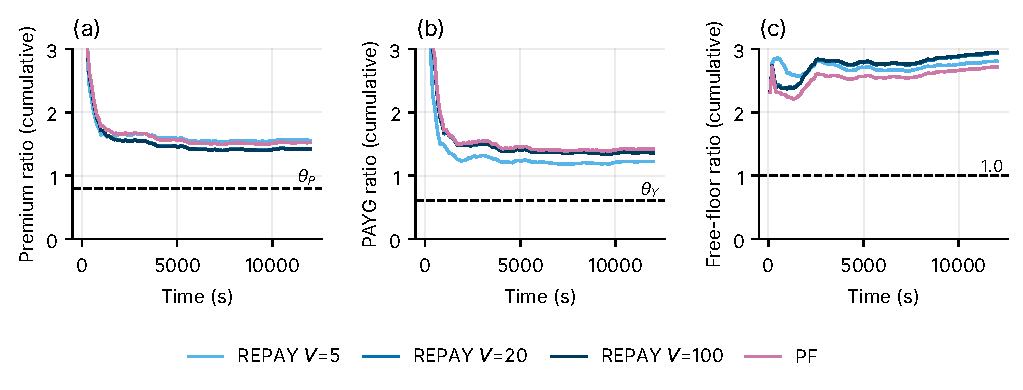
\includegraphics[width=\linewidth]{figures/fig_tiers.pdf}
\caption{Running averages of the three service levels relative to their targets (dashed), default configuration.}
\label{fig:tiers}
\end{figure}

\begin{table}[t]
\centering
\caption{Equal tier weights and demanding targets: the business constraints bind (mean over 5 seeds $\pm$ half-width of the 95\% confidence interval).}
\label{tab:tiers-binding}
\resizebox{0.9\linewidth}{!}{\begin{tabular}{lcccccc}
\toprule
Mechanism & Premium ($\ge 0.8$) & PAYG ($\ge 0.7$) & Free-floor ($\ge 1.0$) & Utility & RT success (\%) & Max envy (Mbit) \\
\midrule
REPAY & $0.819\pm0.012$ & $0.852\pm0.041$ & $2.434\pm0.081$ & $72.89\pm5.68$ & $94.5\pm2.0$ & $16.48\pm1.72$ \\
Plain DPP & $0.821\pm0.013$ & $0.859\pm0.039$ & $2.425\pm0.083$ & $75.23\pm5.68$ & $99.5\pm0.6$ & $1038.51\pm111.09$ \\
PF & $0.549\pm0.023$ & $0.833\pm0.044$ & $3.041\pm0.092$ & $72.61\pm5.24$ & $88.5\pm1.7$ & $0.00\pm0.00$ \\
WFQ & $0.550\pm0.019$ & $0.833\pm0.057$ & $3.038\pm0.089$ & $76.78\pm5.24$ & $100.0\pm0.0$ & $1825.24\pm103.67$ \\
Priority & $0.550\pm0.019$ & $0.833\pm0.057$ & $3.038\pm0.089$ & $76.78\pm5.24$ & $100.0\pm0.0$ & $1825.24\pm103.67$ \\
Credit & $0.551\pm0.028$ & $0.828\pm0.036$ & $3.042\pm0.089$ & $64.58\pm5.34$ & $77.6\pm3.8$ & $120.67\pm46.98$ \\
\bottomrule
\end{tabular}
}
\end{table}

\subsection{Running time}\label{sec:exp-runtime}

The solver performs at most $80$ bisection steps per slot, each a vectorised pass over the devices.
On single-slot instances with $10$ to $3000$ devices the median solve time stays between $1.4$ and $2.0$~ms on one core of a commodity server (Figure~\ref{fig:runtime}); a conic solver applied to the same problem takes $11$ to $27$~ms for $10$ to $300$ devices and agrees with the bisection to a relative difference of $10^{-8}$ in the objective (evaluated at the conic solver's primal point).
The complete allocation step, including rounding and bookkeeping, takes $2.2$~ms per slot at $75$ devices in our simulator, so one-second slots leave more than two orders of magnitude of headroom.

\begin{figure}[t]
\centering
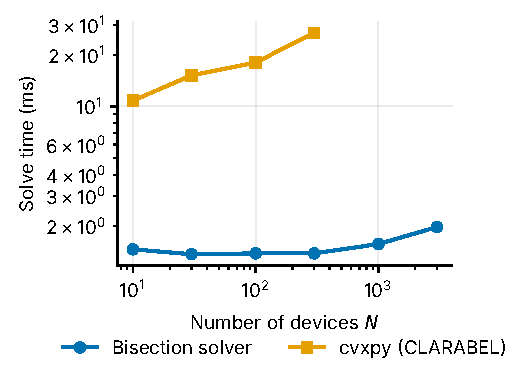
\includegraphics[width=0.45\linewidth]{figures/fig_runtime.pdf}
\caption{Time to solve one slot against the number of active devices.}
\label{fig:runtime}
\end{figure}
